\documentclass[12pt, b5paper,twoside]{tesi_upf}


%CODIFICATION
\usepackage[latin1]{inputenc}


%LENGUAGE
\usepackage[english,catalan]{babel}

%ONLY TO OBTAIN MARK BANK INDEX INDICATION B5
\usepackage[b5paper]{geometry}
\usepackage[cam,a4,center,frame]{crop}

%INCLUDE GRAPHICS AND THE LOGO OF THE UPF
\usepackage{graphicx}

%FONTS TIMES OR GARAMOND, 
\usepackage{times}
%\usepackage{garamond}

%COHERENCE ESTIMATION
\usepackage{graphicx}% Include figure files
\usepackage{dcolumn}% Align table columns on decimal point
\usepackage{bm}% bold math
\usepackage{latexsym}% 
\usepackage{lineno}   
\usepackage{array}
\usepackage{adjustbox}
\usepackage{amsmath,amsfonts,amssymb,amsthm}
\usepackage{newpxtext} 
\usepackage{cite}
\usepackage{booktabs}

%SELD
\DeclareMathOperator{\LL}{\langle}
\DeclareMathOperator{\RR}{\rangle}
\usepackage{graphicx,url,times,booktabs, tabularx}
\usepackage{array}
\usepackage{booktabs}
\usepackage{algorithm, algorithmic}
\usepackage{color}
\usepackage{subcaption}


%WITHOUT HEADINGS: NO MODIFICATION
\pagestyle{plain}

%FOR THE INDEX OF SUBJECTS
\usepackage{makeidx}
\makeindex

%BIBLIOGRAPHY STYLE
\bibliographystyle{apalike}


%SELECT LANGUAGE
\selectlanguage{english}

%THE TABLE OF CONTENTS IS TITLE CONTENTS
%\addto\captionscatalan
  {\renewcommand{\contentsname}{\Large \sffamily Contents}}


%ADD YOUR DATA
\title{Spherical harmonic domain methods for 3D audio production enhancement \todo{(check capitalization)}}
\subtitle{\todo{subtitle Required?}}
\author{Author: Andr�s P�rez L�pez}
\thyear{2020}
\department{of Information and Communication Technologies}
\supervisor{Dr. Adan Garriga Torres\\Dr. Emilia G�mez Guti�rrez}

% TODO
\newcommand\todo[1]{\textcolor{red}{#1}}

% INTEGRAL D
\newcommand{\dif}{\mathop{}\!\mathrm{d}}


\begin{document}


\frontmatter

\maketitle

\cleardoublepage


%%%%%% Dedication

\noindent Write here your dedication \todo{dedication}

\cleardoublepage

%%%%%% End dedication


%%%%%% Thanks
\noindent {\Large \sffamily Thanks} thanks to....  \todo{thanks}

\cleardoublepage

%%%%%% End of thanks

%ABSTRACT IN TWO LEGUAGES.
\selectlanguage{english}
\section*{\Large \sffamily Abstract}
This is the abstract of the thesis in English.  Please, use less
than 150 words. \todo{abstract in english}

\selectlanguage{catalan}
\vspace*{\fill}
\section*{\Large \sffamily  Resum}
Vet aqu� el resum de la tesi en catal�.  Si us plau, utilitzeu
menys de 150 paraules. \todo{abstract in catalan}
\vspace*{\fill}

\cleardoublepage
\selectlanguage{english}
%END OF ABSTRACT

%PREFACE. 
{\bf Preface \todo{is that really needed?}}

\cleardoublepage
%END OF PREFACE


%TABLE OF CONTENTS: REQUIRED
\tableofcontents

%lIST OF FIGURES; ONLY IF THERE ARE FIGURES
\listoffigures
%TO APPER THE LIST OF FIGURES IN THE TABLE OF CONTENTS 
\addcontentsline{toc}{chapter}{List of figures}

%LIST OF TABLES; ONLY IF THERE ARE TABLES
\listoftables
%TO APPEAR THE LIST OF TABLES IN THE TABLE OF CONTENTS
\addcontentsline{toc}{chapter}{List of tables}

%START THE TEXT
\mainmatter

%INSERT CHAPTERS
\chapter{Introduction}

%%%%%%%%%%%%%%%%%%%%%%%%%%%%%%%%%%%%%%%%%%%%%%%%
\section{Motivation}

Ambisonics is a spatial audio theory based on the directional decomposition of the sound field. Conceived in its primal form during the 70s \cite{gerzon1973periphony}, it was not until the 21st century, with a modern mathematical formulation \cite{daniel2000representation} and much more computational power available, that it definitely drew the attention of the research community. 


%\begin{figure}[t]
%  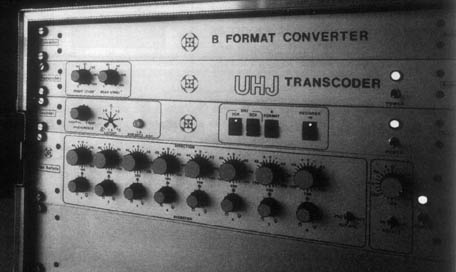
\includegraphics[width=\textwidth]{Figures/Introduction/hardware.jpg}
%    \caption{An ambisonic hardware processor, manufactured by Audio \& Design Recording Ltd. Source: \href{https://commons.wikimedia.org/w/index.php?curid=11813129}{Relen, Wikimedia Commons}}
%  \label{fig:hardware}
%\end{figure}

Nevertheless, the greatest contributor to the current interest in ambisonics has been the rise of Virtual Reality (VR) in recent years.
Although VR focuses primarily on visual cues, the immersive experience can be greatly enhanced by spatial audio \cite{begault20003}. In this context, Ambisonics has been rapidly adopted as \textit{de facto} standard for spatial audio transmission, supposedly due to a variety of factors:

\begin{description}

  \item [Layout independence] As opposed to other audio spatialization techniques that rely on specific playback layouts, ambisonics makes use of an intermediate sound field representation, known as \textit{B-Format} (or just ambisonic audio). This representation, often referred to as \textit{scene-based}, can be then further processed to match any playback configuration. 

  \item [Recording device independence] Regardless of the specific characteristics of an ambisonic microphone, the recorded signal is usually converted into B-Format, which is effectively  the standard exchange format. 

  \item [Ease of manipulations] Signal-independent transformations of the ambisonic stream, and specifically rotations, are computationally inexpensive.

  \item [Binaural transformation] Spatial audio in VR is mostly consumed as binaural; methods for ambisonic to binaural conversion have been known for a long time \cite{noisternig20033d}. Furthermore, VR headsets can easily provide head rotation information, which can be used in combination with scene rotations to provide head-locked audio, which greatly improves localization accuracy and inmersiveness \cite{begault20003}. This is a key feature of ambisonics when compared to static binaural recordings.

\end{description}

Coming back to the issue of the popularity of Virtual Reality, we have selected three events that might epitomize the growth undergone in the second half of the 2010s:

%Coming back to the Virtual Reality popularity, the following three events might be representative of the growth experienced in the second half of the 2010s: 
\begin{enumerate}
	\item The billionaire acquisition by Facebook of the VR headset manufacturer Oculus, in March 2014 \cite{facebookoculus}
	\item \textit{Time} maagazine cover page devoted to VR: \textit{"The surprising joy of Virtual Reality. And why it's about to change the world"} (August 2015) \cite{time};
	\item  M. Zuckerberg's invited talk at the \textit{Samsung Unpacked} event within the World Mobile Congress 2016 in Barcelona: \textit{"VR is the next platform where anyone can experience anything they want"} \cite{bbcnews}.
\end{enumerate}

%(i) the billionaire acquisition by Facebook of the VR headset manufacturer Oculus, in March 2014 \cite{facebookoculus}; 
%(ii) the Time cover page devoted to VR: \textit{"The surprising joy of Virtual Reality. And why it's about to change the world"} (August 2015) \cite{time};
%and (iii) M. Zuckerberg's invited talk at the \textit{Samsung Unpacked} event within the World Mobile Congress 2016 in Barcelona: \textit{"VR is the next platform where anyone can experience anything they want"} \cite{bbcnews}.


\begin{figure}[t!]
\begin{center}
  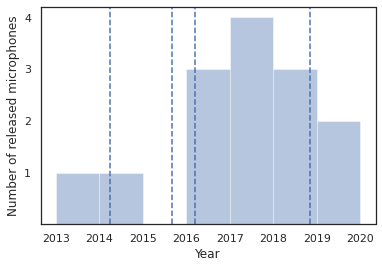
\includegraphics[width=0.8\textwidth]{Figures/Introduction/num_mics_ticks.png}
  \caption{Number of ambisonic microphones released in last years (from \cite{List_of_Ambisonic_hardware}). From left to right, the vertical lines correspond to (1) Oculus acquisition, (2) \textit{Time} cover page on VR, (3) M. Zuckerberg's speech in MWC, and (4) Jaunt announcement of shift towards AR.}
  \label{fig:nummics}
\end{center}
\end{figure}


\begin{table}[t!]
\centering
\caption{List of ambisonic microphones released in recent years (from \cite{List_of_Ambisonic_hardware}).}
\begin{tabular}{cccc}
  \toprule
Manufacturer & Model   & Year & Order \\
\midrule
MH Acoustics & EigenMike   & 2013                     & 4                         \\
Brahma       & (Brahma)                                                   & 2014                     & 1                         \\
Sennheiser   & Ambeo                                                      & 2016                     & 1                         \\
Twirling     & 720 VR    & 2016                     & 1                         \\
Zoom         & H2n                                                        & 2016                     & 1                         \\
Zylia        & ZM-1                                                       & 2017                     & 3                         \\
Twirling     & 720 Lite    & 2017                     & 1                         \\
Ricoh        &  TA-1        & 2017                     & 1                         \\
Nevaton      & Nevaton VR                                                 & 2017                     & 1                         \\
Rode         &  Rode NT-SF1 & 2018                     & 1                         \\
CoreSound    &  OctoMic     & 2018                     & 2                         \\
Zoom         & H3-VR                                                      & 2018                     & 1                         \\
Brahma       & Brahma 8                                                   & 2019                     & 2                         \\
Voyage Audio & Spatial Mic  & 2019    & 2  \\
\bottomrule
\end{tabular}
\label{tab:nummics}
\end{table}


Given this context, many microphone manufacturers and audio-related companies have followed the industry trend in the search for new markets. Only in the interval 2016-2019, 12 different ambisonic microphones have reached the market (Figure~\ref{fig:nummics}) --- a greater amount than all previous existing ambisonic microphones together. A comprehensive list of recent ambisonic microphone releases is shown in \ref{tab:nummics}.

At the present time, however, the high expectations put into VR have significantly lowered, as shown in Figure~\ref{fig:vrfunding}. This is due to a variety of reasons, including lack of interesting content and the high production cost of the headsets \cite{fortune}. The change of focus of Jaunt (formerly one of the biggest VR film production companies) towards Augmented Reality (AR), as of October 2018, might be a paradigmatic example of this tendency \cite{theverge}. 

\begin{figure}[t!]
\begin{center}
  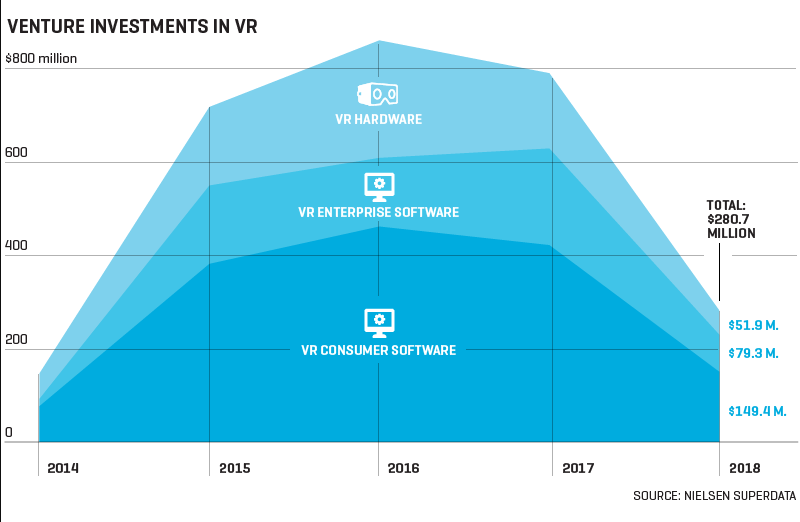
\includegraphics[width=0.8\textwidth]{Figures/Introduction/vr_funding.png}
  \caption{Venture investments in VR in the period 2014-2018. Adapted from \cite{fortune}.}
  \label{fig:vrfunding}
\end{center}
\end{figure}



In any case, the current high availability and affordability of ambisonic microphones brings new challenges from the signal processing perspective. More specifically, ambisonic microphones conform a subset of near-coincident spherical microphone arrays, a category which possesses some specific characteristics.

Although the VR momentum has also reached spherical microphone array processing, many challenges remain still open, and the number of research works specifically focusing on such geometry are low yet. 
Besides that, the growing interest in AR posses new problems related to acoustical signal processing. But since ambisonics is still the standard choice for immersive audio, existing solutions might be successfully adapted. 

Lastly, the advance in signal processing methods for ambisonics can give rise to applications that enhance the work of immersive audio producers, providing meaningful information about the recorded scenes and automating some of the repetitive tasks, thus allowing a more flexible and creative workflow.










%%%%%%%%%%%%%%%%%%%%%%%%%%%%%%%%%%%%%%%%%%%%%%%%
\section{Problem Description}
\label{sec:problemdescription}

The scientific context of the work developed in this thesis is shown in Figure~\ref{fig:scheme1}, which has been inspired by \cite{jarrett2017theory}. 
As we can observe, there are two main topics related with B-Format audio: \textit{generation} and \textit{analysis}, with the signal flow going from the former to the latter.
Although the conceptual approach of the scheme might be very similar for any type of audio, the spatial information conveyed by the ambisonic signal places an emphasis on the informed analysis and description of the sound scene. \\

\begin{figure}[t!]
\begin{center}
  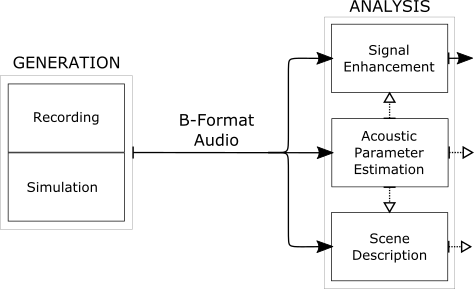
\includegraphics[width=0.8\textwidth]{Figures/Introduction/SCHEME1.png}
  \caption{General scheme of the B-Format audio generation and analysis framework.  Solid lines represent audio signals, while outlined arrows refer to non-audio information.}
  \label{fig:scheme1}
\end{center}
\end{figure}


The problem of B-Format generation is mostly related with dataset generation, which is a common issue for many audio signal processing problems. 
In our case, we consider two different approaches to the data generation problem:
\begin{description}
	\item[Recording] Using spherical microphone arrays for the recording of ambisonic material.
	\item[Simulation] Using numerical methods for the simulation of acoustic scenes.
\end{description}
While recordings are by definition more similar to real scenarios, they are expensive to perform, and can only provide a limited set of parameter possibilities. Simulations, on the other hand, have the potential to cover any desired condition. 
Therefore, it is of our interest to consider the strengths of both signal generation paths.\\


Ambisonic signal analysis has been divided in three categories:
\begin{description}
	\item[Signal Enhancement] Modification of the input signal in order to obtain one or more output signals with desired attributes. 
	
	
	There are a variety of well known signal enhancement problems, including dereverberation \cite{braun2018speech}, source separation \cite{gannot2017consolidated}, or foreground-background segmentation \cite{stefanakis_foreground_2015}. 
	As it has been shown, many of them benefit (or even depend) from the knowledge derived by acoustic parameter estimation methods.
	
	
	\item[Acoustic Parameter Estimation] Low-level analysis of the sound field, which yields quantitative information about different acoustic parameters used to model the acoustic scene.
	
	
	The knowledge about the acoustic parameters of a sound field can be considered either as a goal by itself, or alternatively as a preprocessing step which complements the other analysis categories. Examples of typical estimated acoustic parameters are the \textit{Direction-of-Arrival} (DOA), the sound field diffuseness, or the reverberation time of the enclosure \cite{jarrett2017theory}.  
	
	
	\item[Scene Description] Textual representation of different high-level characteristics of the sound field.
	
	Under the scene description typology we can find a set of applications that provide abstract representations of the sound scene under analysis. Most of the recent research performed in this scope is grouped around the Detection and Classification of Acoustic Scenes and Events (DCASE) community \cite{dcase}. 
	Examples of the problems under consideration are acoustic scene classification \cite{Mesaros2018_DCASE}, sound event localization and detection \cite{Adavanne2018_JSTSP} or audio captioning \cite{drossos2017automated}.
\end{description}





%%%%%%%%%%%%%%%%%%%%%%%%%%%%%%%%%%%%%%%%%%%%%%%%
\section{Scientific Objectives}
\label{sec:objectives}


The list that follows concentrates the main scientific objectives to be developed on this thesis:

\begin{enumerate}
	\item To develop methods for the characterisation of acoustic parameters from recordings originated from ambisonic microphones. 
	\item To propose methodologies for sound event localization and detection in ambisonic domain which are grounded on spatial parametric analysis. 
	\item To contribute to the generation and storage of ambisonic sound scenes, for their usage in controlled experimental environments. 
\end{enumerate}



%%%%%%%%%%%%%%%%%%%%%%%%%%%%%%%%%%%%%%%%%%%%%%%%
\section{Outline}

\begin{figure}[t]
\begin{center}
  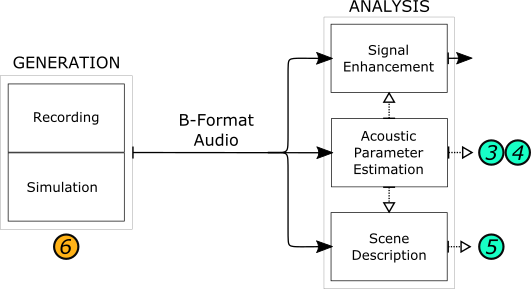
\includegraphics[width=0.8\textwidth]{Figures/Introduction/SCHEME1_NUMBERS.png}
  \caption{General scheme of the B-Format audio generation and analysis framework, including the thesis contributions in form of Chapter numbers.}
  \label{fig:scheme1_numbers}
\end{center}
\end{figure}

The present dissertation is organised as follows. 

\textbf{Chapter~\ref{chap:scientific}} introduces the basic concepts that will be developed throughout this thesis, including spherical harmonics and ambisonics, coherence estimation, parametric analysis or room acoustics. The Chapter also defines the signal models and the mathematical terminology.


Chapters~\ref{chap:rt60}, \ref{chap:coherence} and \ref{chap:seld2019} develop the most significant academic contributions of this thesis. 
\textbf{Chapter~\ref{chap:rt60}} presents a novel method for blind reverberation time in ambisonic recordings. To the best of our knowledge, this is the first method proposal specifically focusing on that problem.   The method is based on a Multichannel Auto-Regressive model of the late reverberation, which allows for an effective dereverberation of the ambisonic sound scene, and enables computation of the reverberation time from an estimation of the room impulse response. The evaluation metrics show a method performance similar to other state-of-the-art methods. The 
 
\textbf{Chapter~\ref{chap:coherence}} analyses the response of tetrahedral microphone arrays, which are the simplest and most common form of ambisonic microphones, under spherically isotropic sound field. The analysis is performed using both simulated and recorded diffuse field, and the results quantify the differences between ideal and real values under a variety of conditions and estimators.  

In \textbf{Chapter~\ref{chap:seld2019}}, a complete system for Sound Event Localization and Detection of ambisonic sound scenes is described. The algorithm comprises two different parts. First, a parametric analysis is performed on the ambisonic signal. The analysis yields spatial localization and temporal activities of the sound events present in the scene. Then, each of those events is assigned to a class label by means of a deep-learning classifier. The method is able to perform in a similar way to the baseline system, while greatly improving its localization capabilities. 
\newpage

Finally, \textbf{Chapter~\ref{chap:data}} presents some libraries and software utilities developed throughout this thesis. All the code has been publicly released under open source licenses. The libraries include utilities for the creation of datasets, the storage and exchange of impulse response files in a standard way, and the implementation of convenience tools for acoustic and microphone array signal processing analysis. Although the libraries do not directly involve any scientific contribution, they can be a great help for scientific and innovative purposes; given the industrial nature of this thesis, we have considered relevant to include them in the present dissertation.\\

In order to provide a schematic representation of the thesis structure and scope, Figure~\ref{fig:scheme1_numbers} features the problem structure stated in Figure~\ref{fig:scheme1}, with the addition of the Chapter numbers with the contributions of this thesis. 



%%%%%%%%%%%%%%%%%%%%%%%%%%%%%%%%%%%%%%%%%%%%%%%%
%\section{Contributions}
%
%
%In the following list we show the main scientific contributions of this dissertation, organised by Chapters:
%
%\begin{itemize}
%
%	\item Chapter 3:\\
%	\textbf{"Blind reverberation time estimation from ambisonic recordings"}.
%	\underline{A. P\'erez-L\'opez}, A. Politis and E. G\'omez.
%	Submitted to \textit{IEEE 22nd International Workshop on Multimedia Signal Processing, 2020.}
%	
%	\item Chapter 4:\\
%	\textbf{"Analysis of spherical isotropic noise fields with an A-Format tetrahedral microphone"}.
%	\underline{A. P\'erez-L\'opez} and N. Stefanakis.
%	\textit{The Journal of the Acoustical Society of America 146.4 (2019): EL329-EL334.}
%
%	\item Chapter 5:\\
%	
%	\textbf{"PAPAFIL: a low complexity sound event localization and detection method with parametric particle filtering and gradient boosting".}
%	\underline{A. P\'erez-L\'opez} and R. Iba�ez-Usach.
%	Submitted to \textit{Detection and Classification of Acoustic Scenes and Events 2020 Workshop (DCASE2020)}.
%	
%	\textbf{"A hybrid parametric-deep learning approach for sound event localization and detection".}
%	\underline{A. P\'erez-L\'opez}, E. Fonseca and X. Serra.
%	In \textit{Proceedings of the Detection and Classification of Acoustic Scenes and Events 2019 Workshop (DCASE2019)}.
%	
%	
%	\item Chapter 6:\\
%	\textbf{"Ambiscaper: A tool for automatic generation and annotation of reverberant ambisonics sound scenes".}\\
%	\underline{A. P\'erez-L\'opez}.
%	In \textit{Proceedings of the 16th International Workshop on Acoustic Signal Enhancement (IWAENC). IEEE, 2018.}
%	
%	\textbf{"Ambisonics directional room impulse response as a new convention of the spatially oriented format for acoustics".}
%	\underline{A. P\'erez-L\'opez} and J. De Muynke.
%	In \textit{Proceedings of the 144th Audio Engineering Society Convention. Audio Engineering Society, 2018.}
%	
%	\textbf{"pysofaconventions, a Python API for SOFA".}
%	\underline{A. P\'erez-L\'opez}.
%	In \textit{Proceedings of the 148th Audio Engineering Society Convention. Audio Engineering Society, 2020.}
%	
%	\textbf{"A Python library for multichannel acoustic signal processing".}
%	\underline{A. P\'erez-L\'opez} and A. Politis.
%	In \textit{Proceedings of the 148th Audio Engineering Society Convention. Audio Engineering Society, 2020.}
%	
%\end{itemize}
%
%Moreover, although not strictly aligned with the research direction of this thesis, the author has collaborated in the following publications:
%
%\begin{itemize}
%	\item \textbf{"Sound event localization and detection based on CRNN using dense rectangular filters and channel rotation data augmentation".}
%	F. Ronchini, D. Arteaga and \underline{A. P\'erez-L\'opez}.
%	Submitted to \textit{Detection and Classification of Acoustic Scenes and Events 2020 Workshop (DCASE2020)}.
%	
%\end{itemize}
%
%
%Finally, as a result of the development of this thesis, the following open-source libraries have been implemented and released. All of them are available through the author's GitHub page \cite{andresgithub}:
%\begin{itemize}
%
%	\item \href{https://github.com/andresperezlopez/ambisonic_rt_estimation}{ambisonic\_rt\_estimation}
%	
%	\item \href{https://github.com/andresperezlopez/DCASE2020}{DCASE2020}
%	
%	\item \href{https://github.com/andresperezlopez/DCASE2019_task3}{DCASE2019\_task3}
%	
%	\item \href{https://github.com/andresperezlopez/masp}{masp: Multichannel Acoustic Signal Processing library}
%
%	\item \href{https://github.com/andresperezlopez/pysofaconventions}{pysofaconventions}
%	
%	\item \href{https://github.com/andresperezlopez/AmbisonicsDRIR}{AmbisonicsDRIR}	
%
%	\item \href{https://github.com/andresperezlopez/ambiscaper}{AmbiScaper} 
%	
%
%
%\end{itemize}




\chapter{Scientific Background}
\label{chap:scientific}

\section{Conventions}
\subsection{Reference system}

In what follows, we will make use of a right-handed coordinate system, where the positive \textit{x}-axis points towards the \textit{front}, the positive \textit{y}-axis points towards the \textit{left}, and the positive \textit{z}-axis points towards the \textit{zenith} (North Pole).

Any position in the unit sphere may be described in spherical coordinates by two angles: the \textit{inclination} angle $\vartheta$, which accounts for the aperture with respect to the \textit{z}-axis, and the \textit{azimuth} angle $\varphi$, which represents the counter-clockwise angle with respect to the \textit{x}-axis from the top-view. 
The value ranges are $0 \leq \vartheta \leq \pi$ for the inclination, and $0 \leq \varphi \leq 2\pi$ for the azimuth. 
The spherical coordinate system used in this thesis is depicted in Figure~\ref{fig:sphericalreference}.

\begin{figure}[h]
\begin{center}
  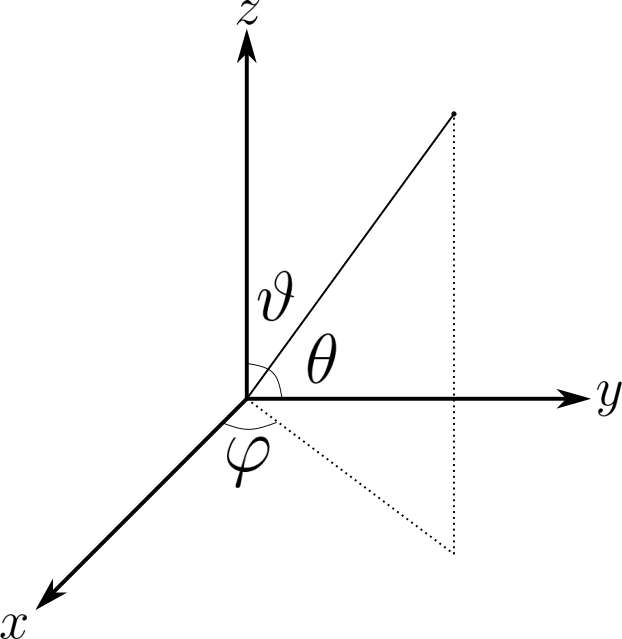
\includegraphics[width=0.5\textwidth]{Figures/ScientificBackground/path829_2.png}
  \caption{Spherical coordinate system used.}
	\label{fig:sphericalreference}
	\end{center}
\end{figure}


Table~\ref{tab:cartesian} shows the spherical coordinate values for some reference points on the unit sphere.
Notice that the poles ($\vartheta = 0, \pi$) are a special case for the spherical coordinate system -- in that case, the azimuth angle is not defined. \\


\begin{table}[hb!]
\centering
\caption{Cartesian and spherical representation of characteristic points along the unit sphere.}
  \begin{tabular}{cccc}
  \toprule
    Position & Cartesian & $\vartheta$ & $\varphi$ \\
\midrule
	front & $[1, 0, 0]$ & $\pi/2$ & $0$ \\
	back & $[-1, 0, 0]$ & $\pi/2$ & $\pi$ \\
	left & $[0, 1, 0]$ & $\pi/2$ & $\pi/2$ \\
	right & $[0, -1, 0]$ & $\pi/2$ & $-\pi/2$ \\
    \textit{zenith} & $[0, 0, 1]$ & $0$ & * \\
    \textit{nadir}  & $[0, 0, -1]$ & $\pi$ & * \\
    \bottomrule
  \end{tabular}
\label{tab:cartesian}
\end{table}

\newpage

The transformation between spherical and cartesian coordinate systems is given by the following relationship:
\begin{equation}
	\begin{aligned}
		x = & \cos{\varphi} \sin{\vartheta}\\
		y = & \sin{\varphi} \sin{\vartheta}\\
		z = & \cos{\vartheta}\\
	\end{aligned}
\end{equation}

The \textit{elevation} angle $\theta$ provides an alternative way of describing the relationship with respect to the \textit{z}-axis. $\theta$ is defined as  the aperture with respect to the \textit{xy}-plane, with positive values towards the positive \textit{z}-axis. The relationship between elevation and inclination angles is:
\begin{equation}
	\theta = \pi/2 - \vartheta
\end{equation}


For the sake of compactness, a point in the unit sphere will be often represented by $\Omega = (\vartheta, \varphi)$.\\

Given the periodic nature of the azimuth angle, the descriptive statistic operations applied to $\varphi$ will refer to the $2\pi$-\textit{periodic} version or the operator; this situation does not affect the inclination/elevation coordinate.


\subsection{Nomenclature}

Throughout the Thesis, we refer to time-domain signals with lowercase, e.g. $x(t)$, with $t$ as the time index. 

Time-domain signals transformed by the Short-Time Fourier Transform (STFT) are represented with uppercase, e.g. $X(k,n)$, where $k \in [0, K-1]$ is the frequency bin index, and $n \in [0, N-1]$ the time frame index. 

Multichannel signals are in general denoted by a subscript variable index, usually with the letter $m$; for example, $x_m(t)$ or $X_m(k,n)$.
Signals with an integer subscript index, such as $x_0(t)$, represent a specific channel of the corresponding multichannel signal.

In the context of ambisonic, subscripts and superscripts are used in signal names with a specific meaning; check Section~\ref{sec:ambisonics} for a detailed explanation.

Vector notation is represented with boldface characters, e.g. $\bm{X}(k,n)$.  When used, the way to construct the vectors will be specified. 



\section{Spherical Harmonics}

\subsection{Definition}

Spherical harmonics are continuous functions defined on the sphere surface. Due to their mathematical properties, any continuously differentiable spherical function can be decomposed as a combination of spherical harmonics, in what is known as the \textit{Spherical Harmonics Expansion} \cite{jarrett2017theory}.




%The spherical harmonic of \textit{order} $\ell>0$ and \textit{degree} $m$, with $|m| <= \ell$  in the direction \Omega is defined as:
Many different spherical harmonic definitions exist in the literature, with minor variations among them. In the following, we will use the real-valued, fully normalized spherical harmonics as defined by \cite{zotter2019ambisonics}: 

\begin{equation}
%ambisonics book 186
	Y_n^m(\varphi, \vartheta) = N_n^{|m|} P_n^{|m|}\cos(\vartheta) \Phi_m(\varphi), 
	\label{eq:sphericalharmonics}
\end{equation}

where the \textit{normalization factor} $N_n^m$ is:

\begin{equation}
%ambisonics book 186
	N_n^m = (-1)^m \sqrt{\frac{2n+1}{2} \frac{(n-m)!}{(n+m)!}}
\end{equation}

the \textit{Legendre polynomials} $P_n^{m}$ are defined as: 

\begin{equation}
%ambisonics book 185
	P_{n+1}^{m} =
	\begin{cases}
 		\frac{2n+1}{n-m+1} x P_n^{m},  &\text{for } n = m,  \\
 		\frac{2n+1}{n-m+1} x P_n^{m} - \frac{n+m}{n-m+1}P_{n-1}^{m} &\text{else}, \\
 	\end{cases}
\end{equation}

with $P_{n}^{n} = \frac{(-1)^n(2n)!}{2^nn!}\sqrt{1-x^{2^n}}$
and the initial term $P_{0}^{0} = 1$, 

and $\Phi_m$ is the azimuthal part of the spherical harmonics: 

\begin{equation}
%ambisonics book 176
	\Phi_m(\varphi) = \frac{1}{\sqrt{2\pi}}
	\begin{cases}
    	\sqrt{2} \sin(|m|\varphi),  &\text{for } m < 0,  \\
    	1,  & \text{for } m = 0,  \\
    	\sqrt{2} \cos(m\varphi),  & \text{for } m > 0.  \\
  	\end{cases}
\end{equation}

\newpage

One of the properties of the spherical harmonics is orthonormality on the sphere surface:

\begin{equation}
	\int_{\mathbb{S}^2} Y_n^m(\varphi, \vartheta) Y_{n'}^{m'}(\varphi, \vartheta) \dif cos{\vartheta} \dif \varphi = \delta_{nn'} \delta_{mm'},
	\label{eq:orthonormality}
\end{equation}

where $\delta_{xy}$ represents the Kronecker delta operator:
\begin{equation}
	\delta_{xy} = \begin{cases}
		1,  &\text{if } x = y,\\
		0,  &\text{else}.
	\end{cases}
\end{equation}

The spherical harmonics depend on the \textit{order} $n \geq 0$ and the \textit{degree} $m$,  $|m| \leq n$ for each value of $n$. In practice, the maximum order $N$, $n \leq N$ determines the spatial resolution of the sound field expansion.\\

Through the spherical harmonic expansion, any sound field may be represented with a limited spatial resolution by the finite combination of all spherical harmonics up to order $N$. 
For a given order $n$, the number of spherical harmonic functions is $2n+1$. With the accumulation of all orders up to $N$, the total number of spherical harmonics is given by $M = (N+1)^2$.
Figure~\ref{fig:sphericalharmonics} depicts all spherical harmonics from orders 0 to 3.

\begin{figure}[hbt]
  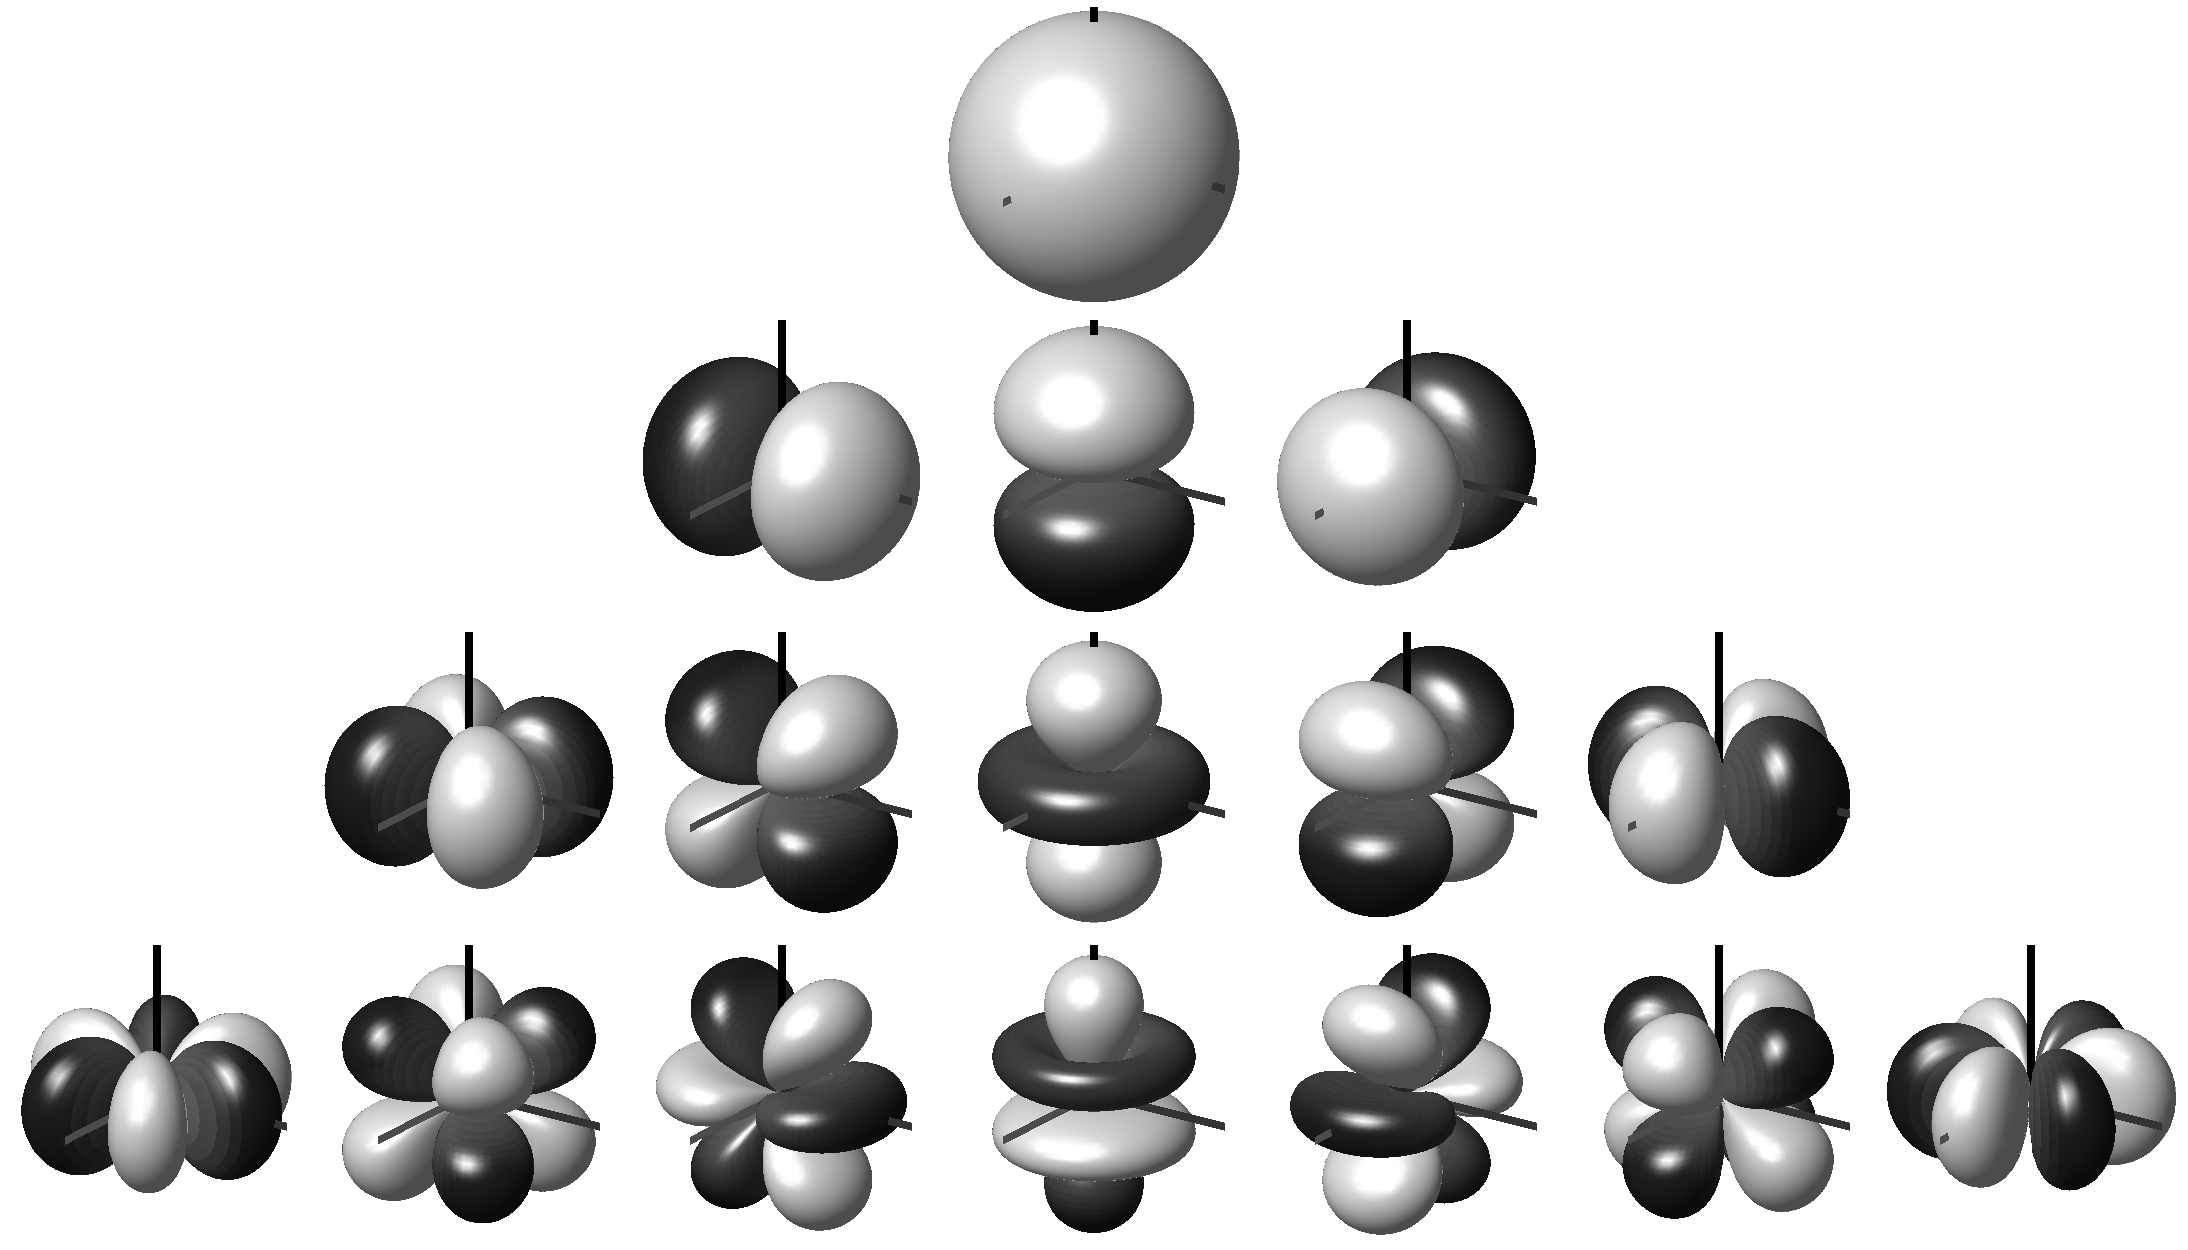
\includegraphics[width=\textwidth]{Figures/ScientificBackground/Spherical_Harmonics_deg3.png}
  \caption{Spherical harmonics up to order $N=3$. The rows correspond to the spherical harmonics of a given order $n$, and the columns span all possible degree values.}
  \label{fig:sphericalharmonics}
\end{figure}


\subsection{Spherical array processing}

Let us consider a sound field captured with a spherical microphone array, which contains $Q$ capsules distributed around a spherical surface of radius $R$ at the positions $\Omega_q, 1 \leq q \leq Q$. 
The captured frequency-domain signals $X_q(k)$ can be represented as the spherical harmonic domain signals $X_n^m(k)$ through the spherical harmonic transform of order $n$ and degree $m$ \cite{moreau20063d}:

\begin{equation}
	X_n^m(k) = \sum_{q=1}^{Q} X_q(k) Y_n^m(\Omega_q) \Gamma_n(kR),
	\label{eq:a2b}
\end{equation}
%\todo{is that actually valid? or Y should be the complex-valued spherical harmonics?}

where the term $\Gamma_n(kR)$ models the radial transfer function, and depends on a number of factors, being the \textit{sphere configuration} one of the most prominent considerations. 
Sphere configuration, in its basic form, refers to the physical properties of the baffle where the capsules are mounted, and it can be either \textit{open} or \textit{rigid}. 
While open configuration is the simplest solution, it might present numerical problems in the form of zeros in its frequency response. Conversely, a rigid baffle interferes with the sound field and might create undesired interferences, but it improves the numerical condition from the open case. Fig.~\ref{fig:magnitude_kr} shows the simulated magnitude response of $\Gamma_n(kR)$  for a spherical array considering both configurations. 
The reader is referred to \cite{moreau20063d} and \cite{rafaely2004analysis}  for a deeper insight into the topic of spherical microphone array design.

%\begin{figure}[h!]
%  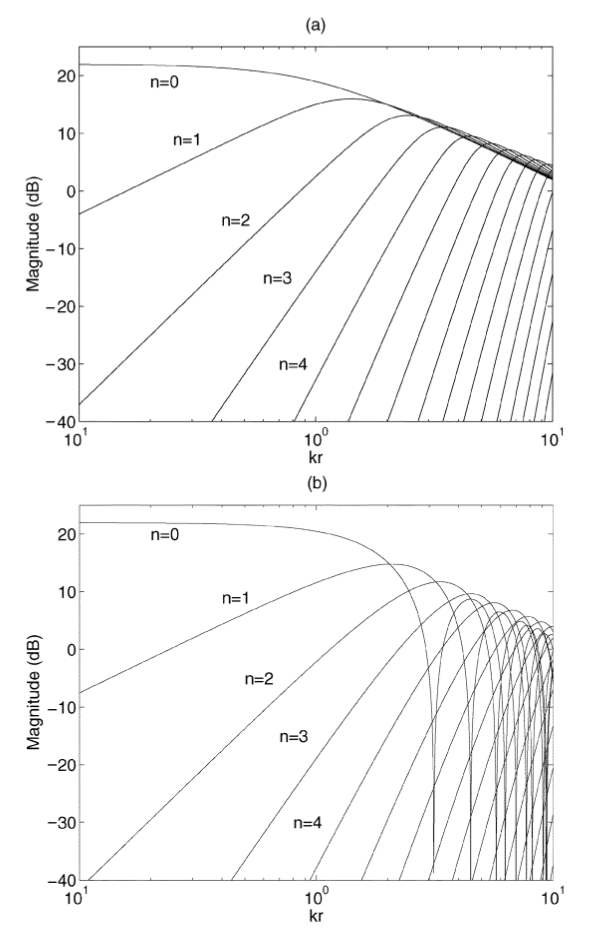
\includegraphics[width=\textwidth]{Figures/ScientificBackground/magnitude_kr.png}  
%  \caption{Magnitude of $\Gamma_n(kR)$ for different ambisonic orders, in the case of (a) rigid sphere, and (b) open sphere configurations. Adapted from \cite{rafaely2004analysis}. }
%  \label{fig:magnitude_kr}
%\end{figure}
%


\begin{figure}[ht]
\begin{center}
  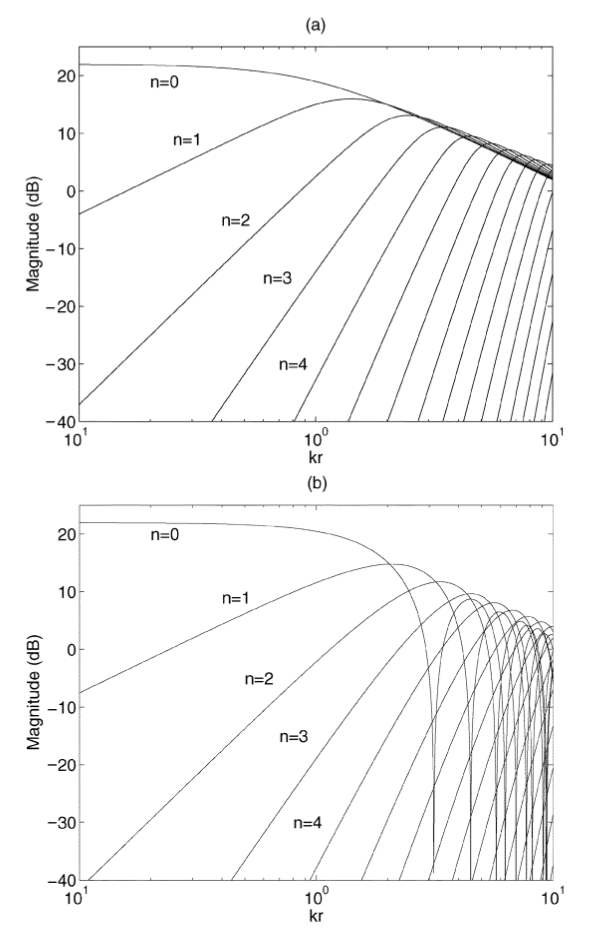
\includegraphics[width=0.5\textwidth]{Figures/ScientificBackground/magnitude_kr.png}
  \caption{Magnitude of $\Gamma_n(kR)$ for different ambisonic orders, in the case of (a) rigid sphere, and (b) open sphere configurations. Adapted from \cite{rafaely2004analysis}. }
	\label{fig:magnitude_kr}
	\end{center}
\end{figure}



%and depends on the microphone geometry, the directivity of the capsules and the physical properties of the baffle where the capsules are mounted.
%
% There are several possible sampling schemes of capsules along the sphere, each one having different properties; the reader is referred to  \cite{rafaely2004analysis} for a deeper insight. \\

\newpage
By using the model from Eq.~\ref{eq:a2b}, the maximum spherical harmonic order $N$ that can be retrieved with negligible spatial aliasing depends on the number of microphone capsules \cite{moreau20063d}:
\begin{equation}
	N \geq (Q + 1)^2.
\end{equation}

\newpage
Furthermore, the sphere radius $R$ has also an effect on the operational bandwidth of the microphone. According to \cite{moreau20063d}, the maximum aliasing-free operational frequency of a spherical microphone array is given by:
\begin{equation}
	f_{max} = \frac{c} {2 R \gamma},
	\label{eq:falias}
\end{equation}

with $c$ being the sound speed, and $\gamma$ the maximum aperture angle between two capsules. 
It is important to notice the existence of a practical minimum frequency of the spherical microphone array, given by the low magnitude in low frequencies of high ambisonic order components, as shown in Fig.~\ref{fig:magnitude_kr}. 



\section{Ambisonics}
\label{sec:ambisonics}

\subsection{Ambisonics Theory}

Ambisonics is a spatial sound recording and playback technology initially developed during the 1970s \cite{gerzon1973periphony}, and further expanded into its modern formulation around the 2000s \cite{daniel2000representation}.  
Ambisonics is based on the idea of decomposing a sound field into its spherical harmonic representation. \\

Originally, the decomposition was limited to first-order spherical harmonics, as the so-called \textit{First Order Ambisonics} (FOA); mainly because of practical limitations. 
The technique was later formalized for arbitrary spherical harmonic orders, known as \textit{Higher Order Ambisonics} (HOA).
In general, with the term \textit{ambisonics} we will be referring to the latter definition.\\

\newpage
\subsubsection{Ambisonic encoding}

Let us consider a sound field composed of a point sound source $S$ located in far-field at the angular position $\Omega_s$. The sound pressure at the coordinate origin $P$ can be expressed in terms of the spherical harmonic expansion of order $N$ as: 
%\todo{check equation, find references, how to explain the domain? extend also to multiple sources by superposition}
\begin{equation}
	P = \sum_{n=0}^{N} \sum_{m=-n}^{n} Y_n^m(\Omega_s) S
	\label{eq:encoding}
\end{equation}


The ordered set of values of all spherical harmonics up to order $N$, evaluated at the source position, is known as the \textit{ambisonic coefficients}:
\begin{equation}
	Y_n^m(\Omega_s) = [Y_0^0(\Omega_s), Y_1^{-1}(\Omega_s),  \ldots ,  Y_N^N(\Omega_s)]
	\label{eq:sphericalharmonicvector}
\end{equation}

Furthermore, the process of multiplying the signal $S$ by the ambisonic coefficients is known in the literature as the \textit{ambisonic encoding}. The resulting signal vector is usually referred to as the \textit{ambisonic} (or \textit{B-Format}) signal $S_n^m$:
\begin{equation}
	S_n^m = Y_n^m(\Omega_s) S
\end{equation}

Note that, because of the superposition principle, a sound field composed of several different point sources can be broken down to the addition of the individual contributions. 

Although the term \textit{B-Format} was initially introduced as an alternative name for first-order ambisonic signals \cite{daniel2000representation}, it is nowadays common to use it as a synonim of ambisonic signals, without any order restriction. We will use the latter acception in what follows.

Historically, the name \textit{B-Format} was used as an opposite of \textit{A-Format}, which describes the signals recorded by a tetrahedral microphone array \cite{gerzon1975design}. The tetrahedron is the simplest and most common form of spherical microphone arrays (indistinctly referred to as ambisonic microphones) with uniform capsule distribution. Again, the term \textit{A-Format} is also currently employed for referring to the signals recorded by any spherical microphone array, regardless of the number or arrangement of capsules.

Likewise, the process of signal conversion from the spatial domain (microphone capsules) to the spherical harmonic domain (ambisonic signals), as in Eq.~\ref{eq:a2b}, is known as \textit{A-B conversion}. A number of different approaches have been developed for this process, and the interested reader is referred to \cite{moreau20063d} for more information.

In practice, there are two alternative ways to generate ambisonic signals. The first one is the \textit{synthesis}, based on the direct application of ambisonics encoding (Eq.~\ref{eq:encoding}) to a monophonic signal. The second one is the \textit{recording} with a spherical microphone array, followed by the aforementioned domain conversion. 


\subsubsection{Ambisonic Decoding}
Conversely, the sound field reconstruction is performed by the \textit{ambisonic decoding} operation. This process is equivalent to weight-and-sum beamforming in the spherical harmonic domain, and it is sometimes also referred to as the \textit{virtual microphone} technique \cite{zotter2019ambisonics}.

Let us consider a loudspeaker located at the angular position $\Omega_p$. In accordance with Eq.~\ref{eq:encoding}, the signal feed $P$ is \textit{decoded} from the ambisonic signal as:
\begin{equation}
	P = \sum_{n=0}^{N} \sum_{m=-n}^{n} Y_n^m(\Omega_s) S Y_n^m(\Omega_\ell)  \alpha_n 
	\label{eq:decoding}
\end{equation}

where $\alpha_n$ is a weighting factor which accounts for the beam directivity.
There are several standard weightings used for different purposes; their values are shown in Table~\ref{tab:alpha}, and the first-order directive patterns are plotted in Figure~\ref{fig:alpha}.

\begin{table}[t]
\caption{Ambisonic decoding: standard values of $alpha_n$ weightings. Adapted from \cite{daniel2000representation}.}
\begin{center}
\begin{tabular}{cccccc}
\toprule
Decoding & $N$ & \multicolumn{4}{c}{$n$} \\ 
&  & 0 & 1 & 2 & 3 \\
\midrule
\textit{basic} & 0 & 1  \\
	& 1 & 1 & 1  \\
 	& 2 & 1 & 1 & 1 \\
 	& 3 & 1 & 1 & 1 & 1 \\
\midrule
\textit{max-rE} & 0 & 0.577  \\
	& 1 & 0.775 & 0.4  \\
 	& 2 & 0.861 & 0.612 & 0.305 \\
 	& 3 & 0.906 & 0.732 & 0.501 & 0.246 \\
\midrule
\textit{in-phase} & 0 & 0.333  \\
	& 1 & 0.5 & 0.1  \\
 	& 2 & 0.6 & 0.2 & 0.029 \\
 	& 3 & 0.667 & 0.286 & 0.071 & 0.008 \\
\bottomrule
\end{tabular}
\label{tab:alpha}
\end{center}
\end{table}

\begin{figure}[htbp]
	\begin{center}
	\begin{minipage}[b]{0.9\linewidth}
		\centerline{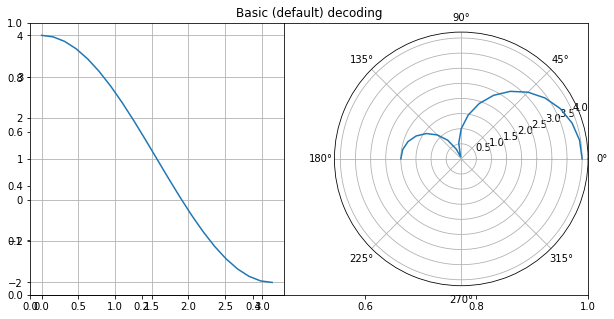
\includegraphics[width=\textwidth]{Figures/Introduction/basic.png}}
	\end{minipage}
	\begin{minipage}[b]{0.9\linewidth}
		\centerline{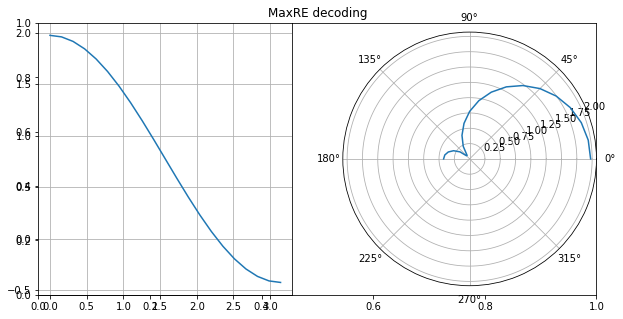
\includegraphics[width=\textwidth]{Figures/Introduction/maxre.png}}
	\end{minipage}
		\begin{minipage}[c]{0.9\linewidth}
		\centerline{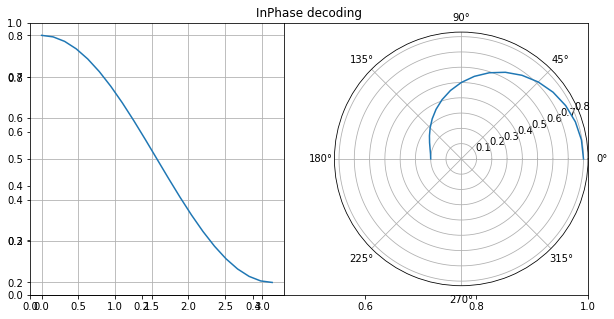
\includegraphics[width=\textwidth]{Figures/Introduction/inphase.png}}
	\end{minipage}
	\caption{Directive patterns of first-order ambisonic decoding.}
	\label{fig:alpha}
	\end{center}
\end{figure}


The decoding equation \ref{eq:decoding} can be written in matrix form as:
\begin{equation}
	P = S_n^m {Y_n^m (\Omega_p)}^T \alpha_n
\label{eq:decodingequation}
\end{equation}

where the superscript $T$ represents the matrix transposition. 
This equation can be extended to the usual case of decoding to a loudspeaker array, comprised of $L$ loudspeakers located at the positions $\Omega_L = [\Omega_{p_1}, \ldots, \Omega_{p_L}]$ . In such case, the loudspeaker feed vector $P_L$ can be written as:
\begin{equation}
	P_L = S_n^m D,
\label{eq:decodingequation2}
\end{equation}
where 
\begin{equation}
	D = \text{diag}(\alpha_n) [{Y_n^{m}(\Omega_{p_1})}^T, \ldots, {Y_n^{m}(\Omega_{p_L})}^T]
\end{equation}

is a $M \times L$ matrix known as the \textit{decoding matrix}, and $\text{diag}(\alpha_n)$ is a diagonal matrix of size $M$ containing the values of $\alpha_n$ along the main diagonal. 
Although the matrix $D$ is frequency-independent and depends solely on the loudspeaker array geometry, in practical scenarios it is usual to include frequency-dependent weightings, $\alpha_n(k)$, to improve the broadband sound field reconstruction \cite{daniel2000representation}.

Furthermore, sound field reconstruction with Eq.~\ref{eq:decodingequation2} is only possible when the loudspeakers are evenly located on the 3D space; in other words, the speaker layout must take the form of one of the five \textit{Platonic solids}: tetrahedron, cube, octahedron, dodecahedron or icosahedron.
Provided that this condition is usually difficult to fulfil in real scenarios, there are several methods which allow ambisonic decoding for such \textit{irregular} layouts. One of the most commonly used is the AllRAD method \cite{zotter2012all}. AllRAD proposes a two step decoding: first, the ambisonic signal is decoded to a nearly-uniform layout of virtual speakers. Then, the signals of the virtual speakers are further distributed into the real speakers by the \textit{Vector-Based Amplitude Panning (VBAP)} method \cite{pulkki1997virtual}.


% The reader is referred to [zotter? daniel? idhoa?] for more information about the vast field of study of ambisonic decoding.






\subsection{Practical considerations}

Due to historical and practical reasons, there are two aspects that must be taking into account when working with ambisonic signals: \textit{channel normalization} and \textit{channel ordering}. 
In the following, the term \textit{channels} will be used as a synonym for spherical harmonics, as they are usually referred to in sound engineering contexts\footnote{In fact, ambisonic signals are inherently multichannel, even though each channel corresponds to a spherical harmonic, and not to a loudspeaker feed as in traditional \textit{channel-based} audio.}.  \\


\subsubsection{Channel normalization}
Let us consider the spherical harmonics $Y_n^m(\Omega)$ as defined in Eq.~\ref{eq:sphericalharmonics}. Due to the orthonormal property showed in Eq.~\ref{eq:orthonormality}, they follow the \textit{fully 3d normalized} or \textit{N3D} channel normalization convention. 
%\todo{what about the 1/sqrt(4pi)???}. 

Alternatively, the \textit{Schmidt 3d semi-normalized} or \textit{SN3D} \cite{daniel2000representation} convention is also of widespread usage. The conversion between \textit{N3D} and \textit{SN3D} is driven by the following expression:
\begin{equation}
	{Y_n^m(\Omega)}^{\text{(N3D)}} = \sqrt{2n+1} {Y_n^m(\Omega)}^{\text{(SN3D)}}
\end{equation}

\textit{MaxN} is another existing convention. It defines all spherical harmonics as having a maximum absolute value of 1: 
\begin{equation}
	\max_{\Omega} |{Y_n^m(\Omega)}^{\text{(MaxN)}}| = 1, \forall (n, m)
\end{equation} 

Finally, the \textit{Furse-Malham} (or \textit{FuMa}) normalization only differs from \textit{Max-N} in the scaling of the zero-th order component: 
\begin{equation}
	{Y_n^m(\Omega)}^{\text{(FuMa)}} = \begin{cases}
		1 / \sqrt{2},  &\text{if } n = 0,\\
		{Y_n^m(\Omega)}^{\text{(MaxN)}},  &\text{else}.
	\end{cases}	
\end{equation} 

Each of the normalization schemes has its own particularities. For instance, \textit{N3D} is the most mathematically straightforward, and spherical harmonics defined in that way can be directly used for both encoding and decoding (as in Eqs~\ref{eq:encoding} and Eq.~\ref{eq:decoding}) -- however, from a sound engineer point of view, other normalization schemes with maximum values below the unity might be preferred, such as \textit{SN3D}. Besides this, \textit{FuMa} has been historically the default normalization \cite{gerzon1985ambisonics}, while the more modern \textit{N3D} and \textit{SN3D} were popularized after J. Daniel's work \cite{daniel2000representation}. \\

\begin{figure}[ht!]
  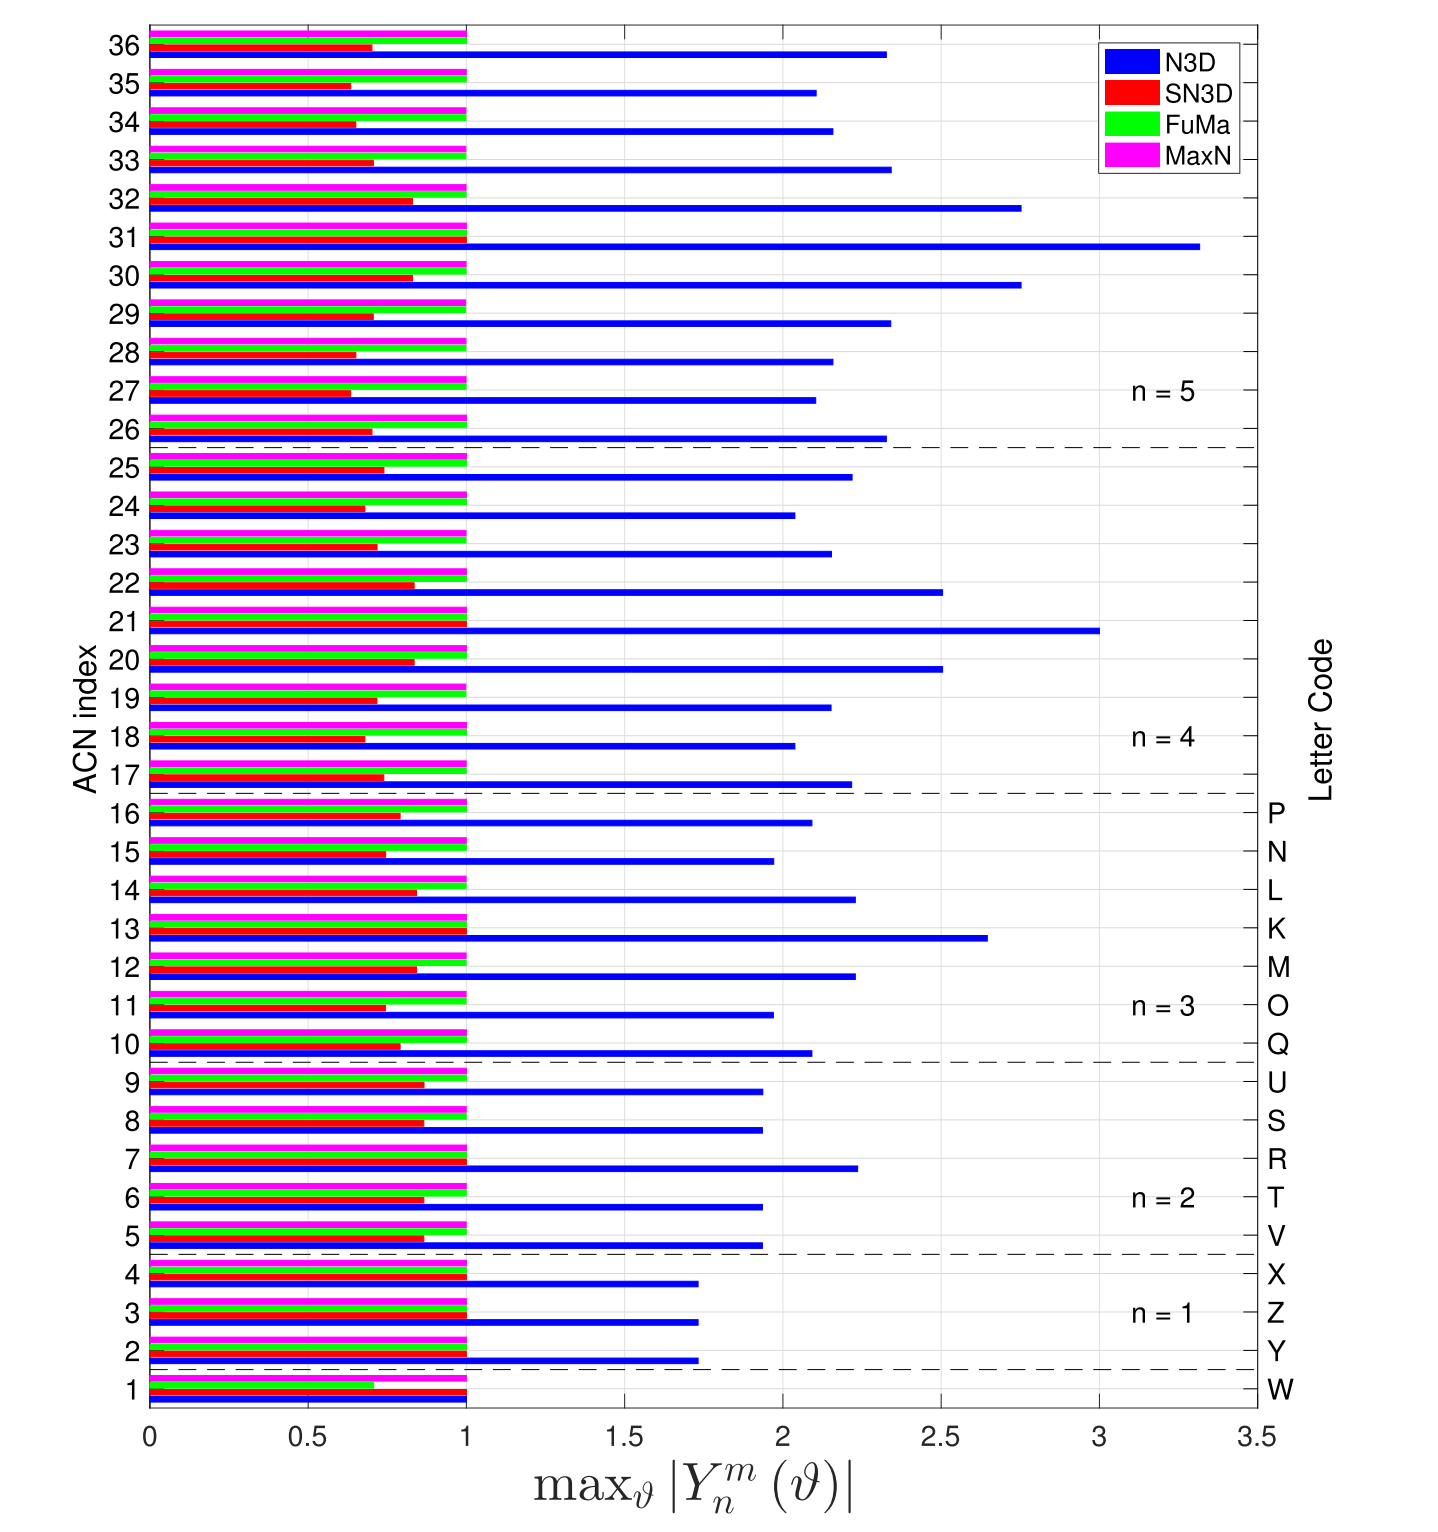
\includegraphics[width=1.1\textwidth]{Figures/ScientificBackground/normalization.png}
  \caption{Maximum value of each ambisonic channel up to order 5, for all different normalization schemes. Image from \cite{carpentier2017ambisonic}.}
  \label{fig:normalization}
\end{figure}


As a summary, Figure~\ref{fig:normalization} displays the different normalization schemes. The reader is referred to \cite{carpentier2017ambisonic} for an extensive review on the topic.


\subsubsection{Channel ordering}

Channel ordering refers to the manner in which spherical harmonics, inherently organized in the 2D space by dimensions $n$ and $m$, are sorted into a one-dimensional vector. 

The \textit{ACN} (from \textit{Ambisonic Channel Number}) scheme follows from the mathematical description given in Eq.~\ref{eq:sphericalharmonicvector}. The spherical harmonics are first ordered by ascending order $n$ and, inside each order, by ascending degree $m$. The index of a given channel $i \in [0 \ldots M-1]$ can be thus obtained by the following relationship:
\begin{equation}
	i = n^2 + n + m 
\end{equation}

Historically, first-order ambisonic audio has followed what it might be called \textit{traditional B-Format} channel ordering \cite{gerzon1985ambisonics}. 
By this scheme, the four channels of a FOA signal $S_n^m$ are referred to by the axis where the corresponding spherical harmonic steers, plus the name $W$ for the zeroth order component:
\begin{equation}
	{S_n^m(\Omega)}^{\text{(FuMa CO)}} = [W, X, Y, Z]
\label{eq:fumaordering}
\end{equation}
where:
\begin{equation}
\begin{aligned}
	&W = S_0^0(\Omega) \\
	&X = S_1^1(\Omega) \\
	&Y = S_1^{-1}(\Omega) \\
	&Z = S_1^0(\Omega)
\end{aligned}	
\end{equation}

This nomenclature was extended to second and third order, and is currently known as the \textit{Furse-Malham} or \textit{FuMa} channel ordering. The channel names use all english alphabet letters from K to Z in third order and, although there would be enough letters to go up to fourth order, the unconvenience of the system was clear \cite{malham2003higher}.
Figure~\ref{fig:normalization} shows the equivalence between \textit{FuMa} (\textit{"letter code"}) and \textit{ACN} channel names.\\

\newpage
In practice, there exist two main combinations of channel normalization and ordering schemes:
\begin{itemize}
  \item The \textit{classical} approach, usually limited to first-order ambisonics, which uses \textit{FuMa} normalization and channel ordering\footnote{In general, it may be expected that \textit{early} ambisonic material follow these conventions without any explicit mention to them.}.
  \item The \textit{modern} approach, inspired by the \textit{ambix} file format [cite ambix], with \textit{SN3D} normalization and \textit{ACN} channel ordering.
\end{itemize}

Anyhow, the \textit{classical B-Format} channel naming and ordering is still widely used when referring to first-order ambisonics. 
%In what follows, we will use indistinctly both \textit{classical} and \textit{ACN} conventions. \todo{is that true?}


\section{Parametric Spatial Audio Analysis}

Trough parametric analysis, sound fields may be described in terms of a small amount of sound sources and associate parameters. Such representation might reduce to a great extent the complexity of processing methods \cite{jarrett2017theory}.


One of the most successful sound field parametric models is DirAC \cite{Pulkki07}, which was originally conceived as a method for impulse response processing and spatial sound reproduction \cite{merimaa2005spatial}.


DirAC (acronym for \textit{Directional Audio Coding}) is a perceptually motivated time-frequency (TF) domain method, based on the assumption that any sound field may be reproduced with high perceptual quality by considering two parameters: the sound field diffuseness and the most prominent sound \textit{Direction-of-Arrival} (DOA) \cite{pulkki2018parametric}. \\


\newpage
Let us consider a \textit{SN3D}-normalized first-order ambisonic signal in time-frequency domain, $S_n^m(k, n)$. 
For the sake of clarity, we will use in this section \textit{FuMa} channel notation and ordering (Eq.~\ref{eq:fumaordering}):
\begin{equation}
	S_n^m(k, n) = [W(k, n), X(k, n), Y(k, n), Z(k, n)]
\end{equation}

Given this representation, we can express the \textit{pressure} $P(k,n)$ of the sound field as:
\begin{equation}
	P(k,n) = W(k,n)
\end{equation}
as well as the sound \textit{pressure-gradient} (or \textit{velocity}) $\pmb{U}(k,n)$ as: 
\begin{equation}
	\pmb{U}(k,n) = - \frac{1}{\rho_0 c} [X(k, n), Y(k, n), Z(k, n)], 
\end{equation}
where $\rho_0$ is the mean medium density, and $c$ is the sound speed. 

The \textit{active intensity} $\pmb{I}(k,n)$, defined as the amount of transmitted acoustic energy, can be expressed in terms of sound pressure and velocity \cite{fahy1990sound}:
\begin{equation}
	\begin{aligned}
	\pmb{I}(k,n) &=  \Re\{P^*(k,n)\pmb{U}(k,n)\} \\
	&= - \frac{1}{\rho_0 c}\Re\{W^*(k,n)[X(k,n),Y(k,n),Z(k,n)]\},
	\end{aligned}
\end{equation}
where $^*$ represents the complex conjugate operator. 

An estimate of the instantaneous DOA $\Omega(k,n)$ can be extracted from the intensity vector, interpreting each of its time-frequency bins as a point in the cartesian space. Effectively, the sound propagation direction is the opposite to the observed arrival direction. 
\begin{equation}
	\Omega(k,n) = \angle(-\pmb{I}(k,n)),
\label{eq:doa}
\end{equation}
with $\angle$ representing the spherical angle operator of a cartesian vector. The result of this computation must be understood as the direction of the net energy flow, which in the case of a single plane-wave will correspond to the source position. \\

Another useful parameter is the \textit{energy density} $E(k,n)$ \cite{stanzial1996reactive}:
\begin{equation}
	\begin{aligned}
		E(k,n) &= \frac{1}{2\rho_0 c^2} |P(k,n)|^2 + \frac{1}{2} {\|\pmb{U}(k,n)\|^2} \\
		&=  \frac{1}{2\rho_0 c^2} \Big(|W(k,n)|^2 + \| [X(k,n), Y(k,n), Z(k,n)] \|^2\Big).
	\end{aligned}
	\label{eq:energydensity}
\end{equation}\\

Finally, the \textit{diffuseness} $\Psi(k,n)$ can be computed from the sound intensity and  energy density \cite{merimaa2005spatial}:
\begin{equation}
	\begin{aligned}
		\Psi(k,n) &= 1 - \frac{ \| \langle \pmb{I}(k,n) \rangle \| }{ c \langle E(k,n) \rangle } \\
		&= 1 - 2\frac{ \| \langle \Re\{W^*(k,n)[X(k,n),Y(k,n),Z(k,n)]\} \rangle \| }{ \langle |W(k,n)|^2 + \| [X(k,n), Y(k,n), Z(k,n)] \|^2 \rangle },
	\end{aligned}
\label{eq:psidefinition}
\end{equation}
 
 where the symbols $\langle \cdot \rangle$ represent the expectation operator, which is usually implemented as time-domain averaging. 

Even though Eq.~\ref{eq:psidefinition} (known as \textit{DirAC's diffuseness}) is one of the most common ambisonic diffuseness estimators, several alternative formulations exist. 
Other diffuseness estimation procedures include the \textit{coefficient of variation method} \cite{ahonen2009diffuseness} and the more recent \textit{COMEDIE} estimator \cite{epain2016spherical}. 
In any case, in what follows, the term \textit{diffuseness} and the symbol $\Psi$ will refer by default to Eq.~\ref{eq:psidefinition}. 

As a mathematical convenience, we will define the \textit{B-Format coherence} as the complement of the diffuseness:
\begin{equation}
	\Delta(k,n) = 1 - \Psi(k,n) 
	\label{eq:delta}
\end{equation}

In conclusion, Figure~\ref{fig:dirac} plots the spectrograms of the DOA $\Omega(k,n)$ and diffuseness $\Psi(k,n)$ of a FOA recording, which consists of a sound source located at the front, plus a moderate amount of reverberation and background noise. 

\begin{figure}[h!]
	\begin{center}
	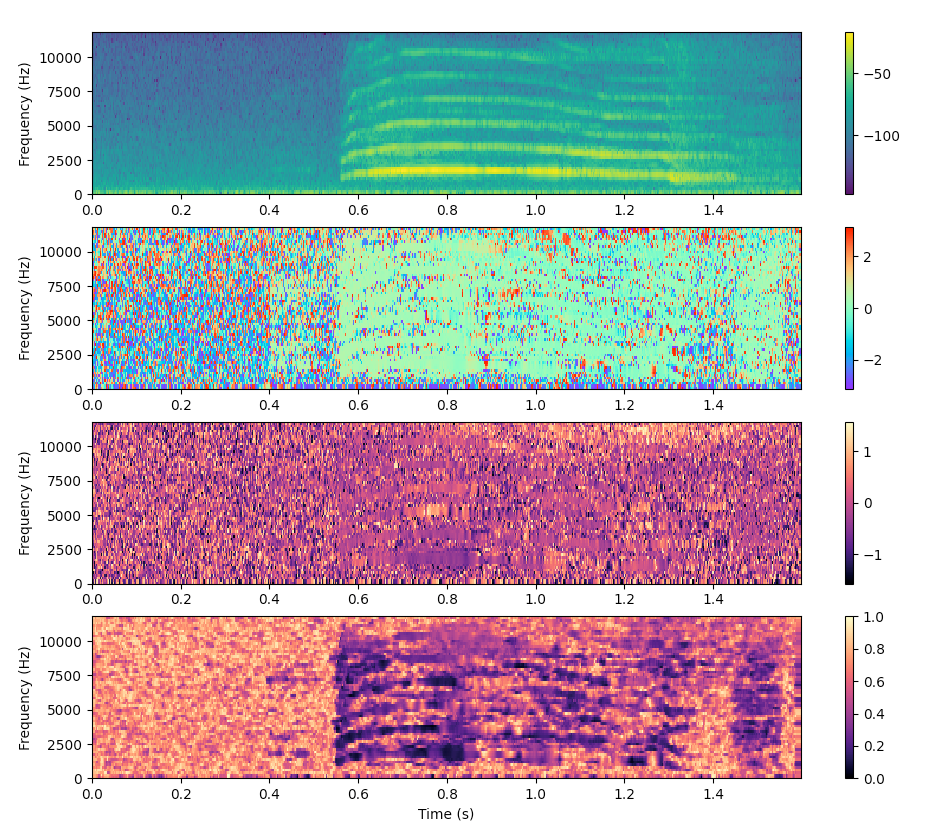
\includegraphics[width=1.1\textwidth]{Figures/Introduction/spectrograms.png}
	\caption{Parametric time-frequency spatial audio analysis of a first order ambisonic recording. From top to bottom: 1.) Magnitude spectrogram of the omnidirectional channel. 2.) and 3.) Azimuth and elevation of the estimated instantaneous narrowband DOAs $\Omega(k,n)$. 4.) Instantaneous narrowband diffuseness $\Psi(k,n)$.}
	\label{fig:dirac}
	\end{center}
\end{figure}




\section{Spatial Coherence Analysis}
%\todo{put this chapter in context or something}\\


In the context of microphone array signal processing, diffuseness is commonly estimated through the
\textit{Magnitude Squared Coherence} (MSC) \cite{elko_spatial_2001} between two frequency-domain signals $S_1$ and $S_2$, as a function of the
\textit{wavenumber} $k$ and the capsule distance $r$:
\begin{equation}
    \text{MSC}_{12}(k r) =
	\frac{|\left\langle S_1(k r) S_2(k r)^* \right\rangle|^2}
	{\left\langle|S_1(k r)|^2\right\rangle \left\langle|S_2(k r)|^2\right\rangle},
    \label{eq:MSC}
\end{equation}
where the $\left\langle \cdot \right\rangle$ operator represents the temporal
expected value, and $^*$ defines the complex conjugate operator. In the case of spherical isotropic noise fields, Eq.~(\ref{eq:MSC})
can be expressed in terms of microphone directivity patterns
$T(\phi,\theta,k r)$ as \cite{elko_spatial_2001}:

\begin{equation}
	\begin{aligned}
&\text{MSC}_{12}(k r) = \frac{|N_{12}(k r)|^2}{|D_{12}(kr)|^2} \\
&= \frac{|\int_{0}^{\pi} \int_{0}^{2\pi} T_1(\phi,\theta,k r) T_2^*(\phi,\theta,k r) e^{-jk r cos\theta} sin\theta d\theta d\phi|^2}{|\sqrt{ \int_{0}^{\pi} \int_{0}^{2\pi} |T_1(\phi,\theta,k r)|^2 sin\theta d\theta d\phi } \sqrt{\int_{0}^{\pi} \int_{0}^{2\pi}|T_2(\phi,\theta,k r)|^2 sin\theta d\theta d\phi}|^2}.
\label{eq:MSCdir}
    \end{aligned}
\end{equation}


Moreover, the general expression of the directivity of a first-order differential microphone is given by the following relationship:

\begin{equation}
	\begin{aligned}
	T_i(\Omega_i) = \alpha_i + (1 - \alpha_i) \cos{\Omega_i},
	\end{aligned}
\end{equation}


where $i \in [1,2]$ is the microphone index, $\Omega_i$ is the angle between wave incidence and microphone orientation axis, and $\alpha_i \in [0,1]$ is the directivity parameter of the microphone $i$, which ranges from bidirectional ($\alpha_i = 0$) to omnidirectional ($\alpha_i = 1$). \\


\newpage
For first-order differential microphones, there is a closed-form expression for the numerator and denominator of Eq.~(\ref{eq:MSCdir}):
\begin{equation}
	\begin{aligned}
    &N_{12}(k r) =  \frac{\alpha_1 \alpha_2 sin(kr)}{kr} \\
    &+ \frac{(1-\alpha_2)(1-\alpha_2)(x_1x_2+y_1y_2)}{(kr)^3}(sin(kr)-kr cos(kr)) \\
    &+ \frac{z_1 z_2}{kr^3}[ ( (kr)^2 sin(kr) + 2kr cos(kr) )(1-\alpha_1)(1-\alpha_2) 
    + 2 sin(kr)(1-\alpha_1)(1-\alpha_2) ] \\
    &+ \frac{z_1}{(kr)^3}[ j(kr)^2 \alpha_2 cos(kr)(\alpha_1-1) + jkr \alpha_2 sin(kr)(1+\alpha_1) ] \\
    &+ \frac{z_2}{(kr)^3}[ j(kr)^2 \alpha_1 cos(kr)(\alpha_2-1) + jkr \alpha_1 sin(kr)(1+\alpha_2) ],\\
    &D_{12}(kr) =  \frac{\sqrt{3 \alpha_1^2+(1-\alpha_1)^2}\sqrt{3 \alpha_2^2+(1-\alpha_2)^2}}{3},
    \label{eq:closedform_msc}
    \end{aligned}
\end{equation}
where $x_i$, $y_i$ and $z_i$ are the cartesian coordinates of the wave incidence angle $\Omega_i = (\varphi_i, \vartheta_i)$.





\section{Reverberation}

In the context of room acoustics, reverberation refers to \textit{"the energy of a sound source that reaches a listener indirectly, by reflecting from surfaces within the surrounding space occupied by the sound source and the listener"} \cite{begault20003}. 
Conversely, in anechoic or free-field conditions, where reverberation is not present, only the direct path of the sound source exists.
Assuming linearity and time-invariance, room reverberation can be fully characterised by its impulse response (IR). \\

Reverberation models often consider two differentiated parts of the reverberant tail, based on both physical and perceptual characteristics: the \textit{early reflections} and the \textit{late reverberation}. 
Early reflections, as the name suggests, refers to the individual sound paths arriving to the listener after a few reflections on the room surfaces, which cause some degree of attenuation. Early reflections typically arrive with a time difference between 1 and 80 ms after the direct path \cite{begault20003}. 
The term late reverberation encompasses all sound paths arriving to the listener after many reflections. Since the temporal density of such reflections increases with time, late reverberation is often modelled in statistical terms.
An schematic representation of a room impulse response (RIR) is shown in Figure~\ref{fig:rir}.\\

\begin{figure}[t!]
	\begin{center}
	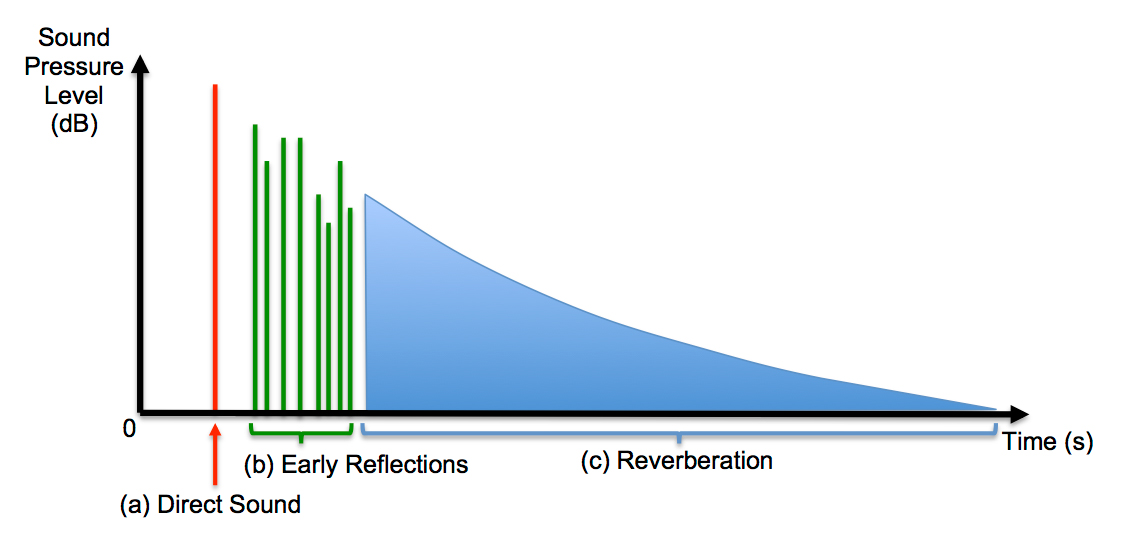
\includegraphics[width=\textwidth]{Figures/Introduction/Acoustic_room_impulse_response.jpg}
	\caption{Room impulse response model, from \cite{murphy2017acoustic}.}
	\label{fig:rir}
	\end{center}
\end{figure}

By following this model, a RIR $h(t)$ can be described as a sequential combination of responses:
\begin{equation}
	h(t) = h_D(t) + h_R(t),
\label{eq:directreverberant}
\end{equation}
where $h_D(t)$ and $h_R(t)$ represent the \textit{direct} (direct path plus early reflections) and \textit{reverberant} (late reverberation) components of the RIR. respectively.

The room impulse response is a function of both the source and the receiver locations. Different levels, delays and directions of direct path and early reflections can obtained from measurements in the same room. However, it is generally assumed that the late reverberation is fixed for a given room, regardless of source/receiver positions. 

Room reverberation plays an important role in psychoacoustics. While early reflections are usually perceived together with the direct path as a single auditory event, due to the \textit{precedence effect} \cite{haas1972influence}, late reverberation has often an influence on the received signal. In the specific case of speech, late reverberation is associated with a loss of intelligibility \cite{braun2018speech}.
In the context of spatial perception, it has been shown that early reflections help the localization and externalization of sources \cite{rudrich2019improving}, while the late reverberation is associated with a spaciousness perception of the room \cite{begault20003}. 


There are a number of measurable parameters which help to characterise room acoustics. 
Perhaps one of the most widespread is the \textit{reverberation time} $T_{60}$ \cite{kuttruff2016room}. It represents the time required for the reverberant sound field power to decay by 60 dB.
Reverberation time can be accurately computed from the room geometry \cite{sabine1927collected} or from the IR \cite{schroeder1965new}.

In the latter case, the $T_{60}$ value is usually estimated from the \textit{Energy Decay Curve} (EDC), which is defined as:

\begin{equation}
	\text{EDC}(t) = 10 \log_{10} \sum_{t'=t}^{\infty} h^2(t),
\end{equation}

where $h(t)$ represents the room impulse response. The values are normalized such that the maximum peak of the curve corresponds to 0 dB.

The EDC is usually modelled as a straight line in logarithmic scale. Therefore, the $T_{60}$ estimation is performed by estimating the slope of a straight line between two reference levels on the EDC time series.
Some of the most used reference levels receive specific names: \textit{Early Decay Time} (EDT), $T_{60}$, and reverberation times $T_{10}$, $T_{20}$ and $T_{30}$. Table\ref{tab:reverberationtimes} shows their correspondent reference levels, where the maximum energy peak is normalized to 0 dB. An schematic representation of the reference levels is depicted in Figure~\ref{fig:reverberationtimes}.

An alternative parameter is the \textit{decay rate} $\alpha_{60}$, which is related to reverberation time $T_{60}$ as:
\begin{equation}
	\alpha_{60} = \frac{3 \ln{(10)}} {T_{60}} (\text{dB/s}).
\end{equation}
 
The decay rate is thus the slope of the EDC curve, in logarithmic scale, expressed in dB per second.  

To conclude, it is important to notice that reverberation time is frequency-dependent. Accordingly, it is usual to report it for octave or third-octave bands, or alternatively to provide its value at a specific frequency. \\


\begin{table}[t]
\caption{Reverberation time computation: usual reference levels}
\begin{center}
\begin{tabular}{ccccc}
\toprule
   & $\text{EDT}$ & $T_{10}$ & $T_{20}$ & $T_{30}$ \\
\midrule
$L_{max} (dB)$ & 0 & -5 & -5 & -5  \\
$L_{min} (dB)$ & -10 & -15 & -25 & -35 \\
\bottomrule
\end{tabular}
\label{tab:reverberationtimes}
\end{center}
\end{table}

\begin{figure}[htbp]
	\begin{center}
	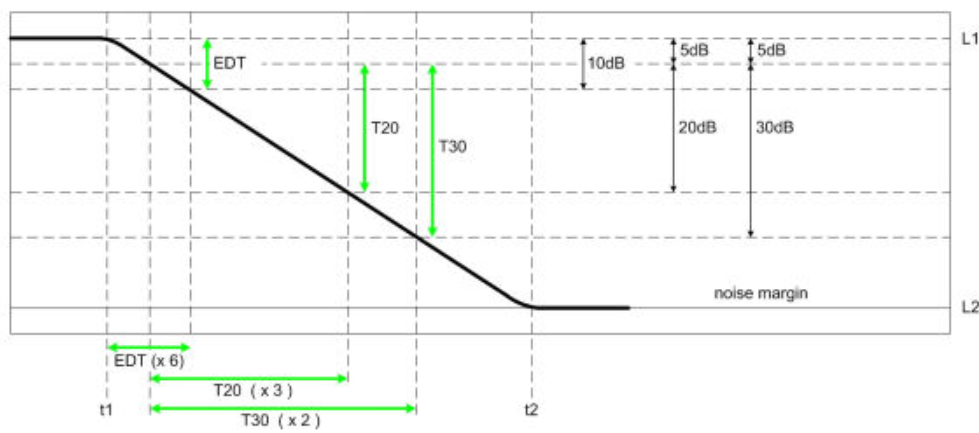
\includegraphics[width=\textwidth]{Figures/Introduction/edt.png}
	\caption{Room impulse response model, adapted from \cite{avinfo}.}
	\label{fig:reverberationtimes}
	\end{center}
\end{figure}


The \textit{Direct to Reverberant Ratio} (DRR) is another relevant acoustic parameter. DDR represents the ratio between direct and reverberant parts of the RIR, as defined in Eq.~\ref{eq:directreverberant}:
\begin{equation}
	DRR = 10 \log_{10} \frac{ \sum_{t=1}^{L_D} h^2_D(t) }{ \sum_{t=1}^{L_R} h^2_R(t)},
\end{equation}
with $L_D$ and $L_R$ as the length of the direct $h_D(t)$ and reverberant $h_R(t)$ filters, respectively.  
At a psychoacoustic level, the direct to reverberant ratio is one of the main cues for distance perception \cite{begault20003}. 

Since the direct path and early reflections (but not the late reverberation) depend on the relative position between source and receiver , the filter $h_D(t)$ and therefore the DRR are as well location-dependent. For a given room, the source-receiver distance that produces a DRR of 0 dB is known as the \textit{critical distance}. 


%\subsection{SOFA Conventions}
%
%The availability of recorded room impulse responses is of great importance to many acoustic signal processing problems. 
%As we have seen, many different RIRs can be obtained from the same room, by just varying the position of the source and the receiver; when the number of source and receiver positions increases, the total amount of measurements increases geometrically. 
%Besides that, the actual format and organisation of the produced data (not only the RIR themselves, but also the source/position annotations) can be arbitrarily different when produced by different groups of people.
%
%In order to overcome potential interoperatibility and reusability issues, the \textit{Spatially Oriented Format for Acoustics} (SOFA) convention \cite{majdak2013spatially}, also known as the \textit{AES-69} standard \cite{majdak2015aes69}, proposes a unified file format for the storage of IR-related data. 
%Despite that SOFA was initially created with a focus on \textit{Head-Related Impulse Response} (HRIR) data, its structure is very convenient to any kind of multi-location impulse responses, including ambisonics.


%\todo{RIR SIMULATION: IMAGE METHOD?}


\section{Signal Models}


Let us consider a sound source represented by the signal $s(t)$, located in a given acoustic enclosure characterised by its room impulse response $h(t)$. The resulting reverberant signal $x(t)$ can be therefore described as the \textit{convolutive mixture} of the source and the RIR: 
\begin{equation}
	x(t) = s(t) \ast h(t).
\label{eq:convolutivemixture}
\end{equation}

\newpage
When dealing with multichannel room impulse responses, as it is the case in ambisonics, the multichannel reverberant signal $x_m(t)$ is obtained by the convolutive mixture of each RIR channel independently:
\begin{equation}
	x_m(t) = s(t) \ast h_m(t).
\label{eq:convolutivemixturemultichannel}
\end{equation}

The time domain convolution operation, under certain assumptions, is equivalent to the multiplication in frequency domain. By doing so, Eq.~\ref{eq:convolutivemixture} can be expressed as:
\begin{equation}
	X(k,n) = S(k,n) H(k,n).
\label{eq:multiplicativetransferfunction}
\end{equation}

Eq.~\ref{eq:multiplicativetransferfunction}, also known as the \textit{Multiplicative Transfer Function (MTF) model} is only valid when the length of the filter $h(t)$ is smaller than the length of the analysis window used in the STFT. 


On the contrary, when the filter $h(t)$ spans across several analysis windows, the resulting model is referred to as the \textit{Convolutive Transfer Function (CTF) model}:
\begin{equation}
	X(k, n) = \sum_{l=0}^{L_h-1} H(k, l) S(k, n-l), 
\label{eq:convolutivetransferfunction}
\end{equation} 
where $L_h$ is the length of the filter $H(k, n)$ in time frames. 



%\todo{isotropic noise}



%\section{Practical Considerations}
% TODO I don't remember what is this


\chapter{Coherence Estimation}



\section{Introduction}

A number of practical applications benefit of the knowledge about the diffuseness of a sound field, including speech enhancement and dereverberation \cite{p_habets_dual-microphone_2006}, noise suppression \cite{ito_designing_2010}, source separation \cite{duong_under-determined_2009} or background estimation \cite{stefanakis_foreground_2015}. In the field of spatial audio, diffuseness estimation is often used for parametrization \cite{pulkki_directional_2006, politis_compass_2018}, Direction-of-Arrival estimation \cite{thiergart_localization_2009} or source separation \cite{motlicek_real-time_2013}.

\todo{In this chapter}, we study diffuseness estimation by subjecting a tetrahedral microphone array to spherically isotropic noise fields.
The motivation for this work is, first, that tetrahedral arrays are a well known type of microphone arrays, which have today become popular for applications related to Virtual and Augmented Reality. 
Second, the spherical isotropic sound field is known to be a good approximation to the reverberant part of the sound field in a room \cite{elko_spatial_2001, mccowan_microphone_2003}, and therefore it would be interesting to investigate how different microphone arrays behave under such conditions.




\subsection{Problem definition}

Under spherical isotropic noise, the theoretical coherence between any pair of zeroth- and first-order ambisonic virtual microphones is equal to 0 for all frequencies, due to the spherical harmonic orthogonality (Eq.~\ref{eq:orthonormality}) \cite{elko_spatial_2001}. This result can also be assessed by Eq.~(\ref{eq:closedform_msc}).

However, there are several practical factors that might corrupt the coherence estimation, such as the approximation of the temporal expectation by time averaging \cite{thiergart_diffuseness_2011} in Eq.~(\ref{eq:psidefinition}), or the non-ideal implementation of the radial filters $\Gamma_n(kR)$ (Eq.~\ref{eq:a2b}) for the \textit{A-B conversion}\cite{schorkhuber_ambisonic_2017}.

In the following sections, we present several experiments that illustrate the behavior of different coherence estimators applied on the signals captured with a tetrahedral microphone subjected to spherical isotropic noise, using both simulated and real sound recordings.



\section{Methods}

\subsection{Simulation}
Spherical isotropic noise has been generated following the \textit{geometrical method} \cite{habets_generating_2007, habets_comments_2010}, using $I = 1024$ plane waves. The resulting \textit{A-Format} signals correspond to a virtual tetrahedral microphone array mimicking the Ambeo\footnote{Sennheiser Ambeo VR Mic. 
\todo{https://en-us.sennheiser.com/microphone-3d-audio-ambeo-vr-mic}}
characteristics ($R=0.015$ meter, $\alpha=0.5$). 
The generated audio has a duration of 60 seconds. 





\subsection{Recording}

Spherical isotropic noise has been rendered to a spherical loudspeaker layout with 25 \textit{Genelec 8040}. The loudspeakers are arranged into three azimuth-equidistant 8-speaker rings at inclinations $\vartheta = [\pi/4, \pi/2, 3\pi/4]$, plus one speaker at the zenith.
The different speaker distances to the center are delay- and gain-corrected, and the signal feeds are equalized to compensate for speaker coloration. The room has an approximate $T_{60}$ of 300 ms measured at the 1 kHz third-band octave. 

The spherical isotropic noise has been also created by the \textit{geometrical method}, encoding a number of uncorrelated noise plane waves in ambisonics with varying orders $N \in [1,5]$. Due to practical limitations related with the software, the minimum number of sources $I = 256$ for an accurate sound field reconstruction \cite{habets_comments_2010} could not be reached - instead, the analysis has been performed parametrically with $I = [8, 16, 32, 64]$.
For each value of $N$ and $I$, approximately 15 seconds of audio have been recorded with an Ambeo microphone located at the center of the speaker array.

Ambisonics decoding is performed with an AllRAD decoder, passing through a spherical 64-point 10-design virtual speaker layout, and includes an imaginary speaker at the nadir. The decoding matrix uses \textit{in-phase} weights.



\subsection{Data processing and metrics}

The sampling rate of all signals is 48 kHz.
All frequency-domain results have been obtained by averaging their time-frequency representations over time.  
\textit{A-B conversion} has been computed using \textit{Ambeo A-B converter} AU plugin, version 1.2.1.

Two error metrics are considered: the frequency-dependent squared error $\varepsilon(k)$:
\begin{equation}
	\varepsilon(k) = |X_1(k) - X_2(k)|^2,
	\label{eq:mse}
\end{equation}

 and the mean squared error $\bar{\varepsilon}$:

\begin{equation}
    \bar{\varepsilon} = \frac{1}{K}{\sum_{k=1}^{K} |X_1(k) - X_2(k)|^2}
    \label{eq:nmse}
\end{equation}



\section{Results and discussion}
\subsection{\label{subsec:results_aformat}A-Format}

\begin{figure}
	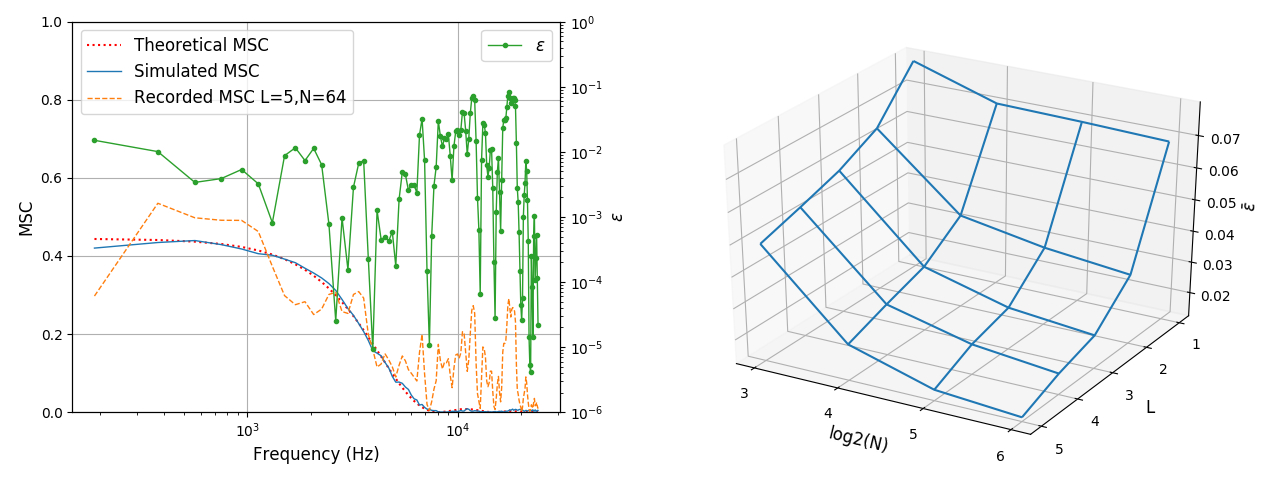
\includegraphics[width=\textwidth]{Figures/CoherenceEstimation/Figure1}
    \caption{\label{fig:Fig1}\textit{A-Format} coherence between microphone signals. Left: $\text{MSC}$ as a function of the frequency of theoretical, simulated and recorded \textit{((BLD,BRU)},  $N=5, I=64$) signals. Right: mean error $\bar{\varepsilon}$ of the recorded signals' $MSC$ \textit{(BLD,BRU)} compared to the simulated values, for all values of $N$ and $I$.\todo{REDO FIGURE WITH N AND I}}
\end{figure}


The coherence of the generated \textit{A-Format} signals is exemplified in Fig.~\ref{fig:Fig1} (left), which shows the $MSC$ between the capsule pair (\textit{BLD,BRU}) for the theoretical, simulated and recorded cases.
The theoretical coherence is derived from Eq.~(\ref{eq:closedform_msc}), while simulated and recorded MSC have been computed by Welch's method, using a \textit{hanning} window of 256 samples and 1/2 overlap.
The difference between theoretical and simulated coherence is negligible for practical applications.
However, there is a noticeable difference when compared to the recorded coherence. 
In general, the recorded $\text{MSC}$ follows the tendency of the simulated curve up to around 5 kHz.
Above this frequency, the recorded $MSC$ presents several spectral peaks, which might be partially explained by the interference of the microphone itself in the recorded sound field, and by the non-ideal directivity of the capsules.
The squared error $\varepsilon(k)$ with respect to the simulated curve is shown in Fig.~\ref{fig:Fig1} (left), while Fig.~\ref{fig:Fig1} (right) represents the same error averaged over frequency $\bar{\varepsilon}$ for different spatial resolution values of the diffuse field reproduction algorithm.
As expected, $\bar{\varepsilon}$ decreases with increasing values of $N$ and $I$.




\subsection{B-Format} 
\begin{figure}
	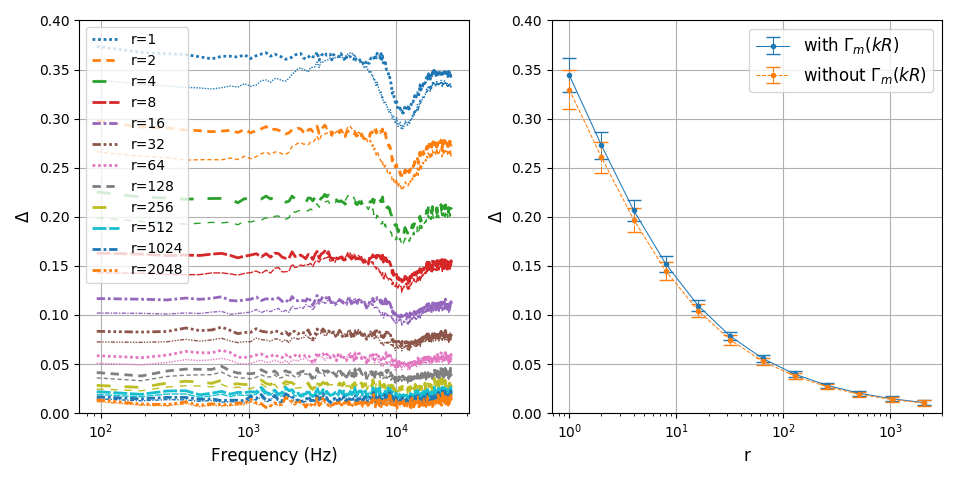
\includegraphics[width=\textwidth]{Figures/CoherenceEstimation/Figure2}
	\caption{\label{fig:Fig2} Estimated \textit{B-Format} coherence ($\Delta$) of a simulated diffuse sound field, as a function of the temporal averaging vicinity radius $r$. Left: $\Delta(k)$ for different values of $r$, with (coarse) and without (fine) application of radial filters. Right: mean and standard deviation of $\Delta(k)$ as a function of $r$.}
\end{figure}

In order to evaluate the dependency of the \textit{B-Format coherence} $\Delta$ on the number of time frames used for averaging, the following procedure is presented.
The simulated \textit{A-Format} sound field has been transformed into the spherical harmonic domain, with and without the application of radial filters $\Gamma_n(kR)$ (Eq.~\ref{eq:a2b}). Then, $\Delta$ has been computed with Eq.~(\ref{eq:delta}) for exponentially growing values of $r$ between 1 (8 ms) and 2048 (10.92 s), where $r$ is the vicinity radius used for time averaging, and the number of time windows is given by $T = 2r+1$.
The time-frequency representation is derived by applying the STFT with the same window parameters as in Subsection \ref{subsec:results_aformat}.\\

Figure~\ref{fig:Fig2} (left) shows the great dependence of $\Delta$ on $r$.  The estimated coherence tends to the theoretical values with increasing values of $r$. This tendency is better appreciated in Fig.~\ref{fig:Fig2} (right): the curve asymptotically decreases to a value $\Delta_{min}\approx0$.

Another interesting observation comes from the frequency response of the curves. For all values of $r$, the coherence of the compensated \textit{B-Format} signal (with $\Gamma_m(kR)$) is roughly flat up to around 7 kHz, which approximately corresponds to the operational spatial frequency range of the microphone \cite{gerzon_design_1975}.
Above this value, the coherence response looses the flatness due to spatial aliasing (Eq.~\ref{eq:falias}). The response above the maximum frequency could be stabilized, if needed, by alternative diffuseness estimation methods \cite{politis_direction--arrival_2015}.

The coherence level differences along frequency are inversely proportional to $r$ --- the effect is better depicted by the standard deviation values (right).
The effect of the radial filters in the coherence measurement is also shown: for a given $r$, the shape of the coherence is always less flat if no filters are applied. Conversely, in this case, coherence values are always smaller for the same $r$. This effect might be explained taking into account the inter-channel coherence introduced by microphone and encoder imperfections in real scenarios \cite{schorkhuber_ambisonic_2017}.

As a remark, the comparison between Figs.~\ref{fig:Fig1} and \ref{fig:Fig2} provides evidence that the application of the spherical harmonic transform might be able to yield more accurate diffuseness estimations, due to a better signal conditioning \cite{epain_spherical_2016}.\\



\begin{figure}
	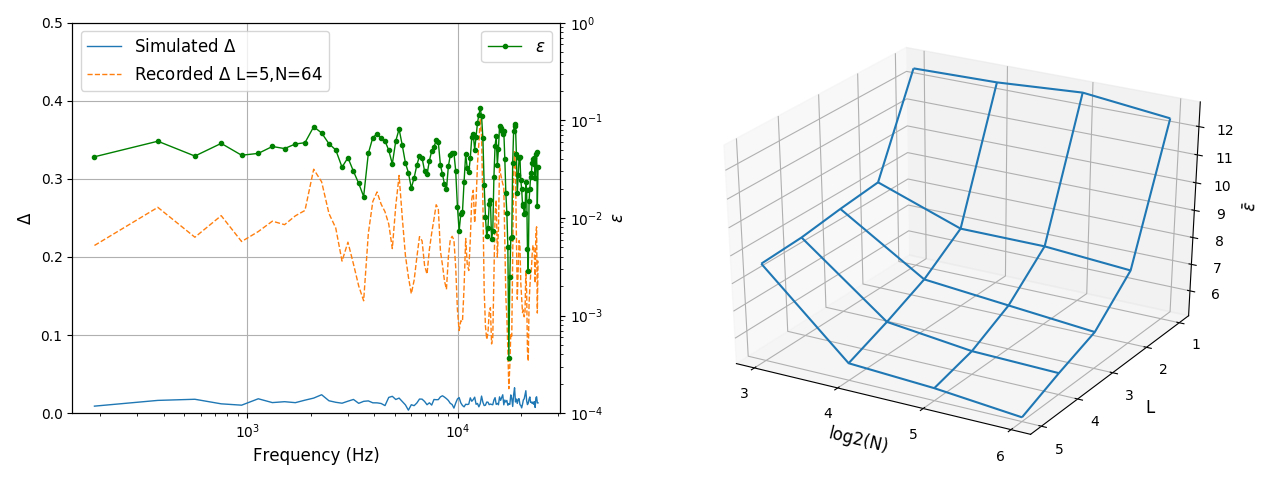
\includegraphics[width=\textwidth]{Figures/CoherenceEstimation/Figure3}
	\caption{\label{fig:Fig3}\textit{B-Format coherence} between microphone signals. Left: $\Delta$ of simulated and recorded ($N=5, I=64$) signals. Right: $\bar{\varepsilon}$ of the recorded signals coherence across all values of $N$ and $I$.\todo{REDO FIGURE} }
\end{figure}

Figure~\ref{fig:Fig3} (left) shows the estimated coherence for the recorded sound field with $N=5$ and $I=64$, using a vicinity radius of $r=1024$ ($\approx$ 5 s).
The curve is centred around $\Delta=0.25$ and presents several spectral peaks, as in the \textit{A-Format} case. 
It is important to notice here that the deviations between the coherence of the simulated and the recorded sound fields are much stronger compared to those of Fig.~\ref{fig:Fig1}. 

This effect can be also appreciated in Fig.~\ref{fig:Fig3} (right): the mean squared error is around two orders of magnitude higher in \textit{B-Format}.
Nevertheless, similar as in Fig.~\ref{fig:Fig1} (right), $\bar{\varepsilon}$ decreases with increasing values of $N$ and $I$.
This behavior suggests that the deviations between the recorded and the simulated coherence can be to a large degree explained by the low spatial resolution of the reproduction system; given a higher number of loudspeakers, we expect that the reproduced diffuseness will tend to the theoretical expression.




\section{Conclusions}
The diffuseness of a sound field is an important parameter for several applications. In this work, two different metrics of diffuseness have been defined and measured with a tetrahedral microphone subjected to spherical isotropic noise.

The analysis shows, first, the impact of the time-averaging window length on the \textit{B-Format} diffuseness estimator.
This result might be useful for designing coherence estimators that are parametrized with respect to the length of the analysis window \cite{thiergart_diffuseness_2011}.

Second, the feasibility of diffuse sound field reproduction by a spherical loudspeaker array using ambisonics plane-wave encoding and the \textit{geometrical method} is studied. 
Results suggest that this approach is viable, given a sufficient spatial resolution; a quantification of the impact of the number of loudspeakers remains for future work.





\chapter{Autoregressive Impulse Response Models}
\chapter{Sound Event Localization and Detection}
\chapter{Data generation and storage}



Explain about mono files plus ambisonics IRs.


\section{Recorded IRs}

AmbisonicsDRIR: explain problematics, standard, etc.
also: pysofaconventions


\section{Simulated IRs}

explain different methods and libraries.
tell about masp.


\section{High-level scene description}

ambiscaper





\chapter{Conclusions}


\section{Summary of Contributions}

In this thesis we have presented our contributions to different components of an ambisonics analysis and generation framework, with a focus on reproducibility and portability to real-world scenarios.
The main scientific objectives of this thesis, as they were described in Section \ref{sec:objectives}, are: 
 

\begin{enumerate}
	\item The development of methods to support and improve the characterization of acoustic parameters.
	\item The research on parametric-based methodologies for sound event localization and detection.
	\item The contribution in the generation and storage of annotated ambisonic datasets.
\end{enumerate}

In what follows, we summarize the main contributions of the present thesis, both in the academic and software scopes.

%  \begin{itemize}

%  	 \item Blind reverberation time estimation
\newpage
\paragraph{Blind reverberation time estimation}
Chapter~\ref{chap:rt60} presents a novel methodology for the blind estimation of reverberation time from ambisonic audio. The method is based on two main steps: first, dereverberation using a multichannel auto-recursive model (MAR), and second, estimation of the  filter from reverberant and dereverberated signals. The actual reverberation time value is estimated from the energy decay of the estimated filter. 

The proposed system is the first attempt in the literature to address the blind reverberation time estimation problem specifically for ambisonic signals. Compared with a state-of-the-art monophonic estimator, our method is able to improve in all the evaluation metrics under consideration.


\paragraph{Coherence estimation}
In Chapter~\ref{chap:coherence}, we have characterised the response of tetrahedral microphones to isotropic noise field, which is one of the most used models for diffuse sound. Furthermore, the capabilities of a spherical loudspeaker array with respect to the reconstruction of diffuse sound fields using ambisonics are also quantitatively analyzed.

\paragraph{Sound event localization and detection}
Chapter~\ref{chap:seld2019} describes an algorithm for sound event localization and detection (SELD), developed in the context of the DCASE 2020 challenge. The method estimates the localization and temporal activity of the sound events based on a particle filter that tracks event trajectories obtained from the parametric analysis of the ambisonic sound field. Each event is assigned to a sound class by a machine learning classifier that uses low- and mid- level audio features. 

Results show a significant performance increase in all evaluation metrics under consideration, compared with a state-of-the-art deep learning baseline.
This suggests that our approach, substantially different to the baseline and the majority of state-of-the-art methods, represents a feasible alternative in situations with low-complexity or small database constraints. 


\paragraph{Data generation and management}
Finally, the thesis contributions to more practical aspects are presented in Chapter~\ref{chap:data}. Those contributions comprise two software libraries written in Python: one of them focused on spherical microphone array and acoustic simulation, and another one implementing the SOFA standard, which has also been revised and modified for allowing the representation of ambisonic data. 
Finally, a novel software tool for the procedural creation of annotated reverberant ambisonic datasets has ben also presented.

%  	\begin{description}
%  		\item [1. Parameter estimation] Novel technique for blind RT60 estimation of ambisonic recordings from autoregressive models.
%	\end{description}
%
%  
%  	\item Coherence estimation (Chapter~\ref{chap:coherence}):
%  	\begin{description}
%  		\item [1. Parameter estimation] Contribution to the characterization of coherence with tetrahedral microphones (the most common spherical arrangement).
%	\end{description}
%
%
%  	\item Sound Event Localization and Detection (Chapter~\ref{chap:seld2019}):
%  	\begin{description}
%  		\item [2. Scene Description]: Novel state-of-the-Art methodology for Sound Event Localization and Detection	.
%  	\end{description}
%  	
%  	\item Data generation and storage (Chapter~\ref{chap:data}):
%  		\begin{description}
%  			\item [3. Data Generation]: Library for acoustic simulation and spherical microphone array processing.
%  			\item [3. Data Generation]: Proposal and implementation of a file convention for the storage of recorded ambisonic RIRs.
%  			\item [3. Data Generation]: Novel tool for high-level description and generation of of ambisonic datasets.
%
% 		\end{description}
%
%  \end{itemize}
  
   
%Figure~\ref{fig:scheme1_numbers2}, which is a copy of Figure~\ref{fig:scheme1_numbers}, 
% has been included here again in order to help the contextualization of the contributions. 
%
%  \begin{figure}[h!]
%  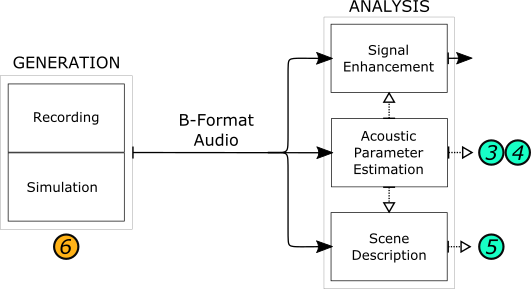
\includegraphics[width=\textwidth]{Figures/Introduction/SCHEME1_NUMBERS.png}
%  \caption{General scheme of the B-Format audio generation and analysis framework, including the thesis contributions in form of Chapter numbers.}
%  \label{fig:scheme1_numbers2}
%\end{figure}




\section{Future Work}

This thesis has tackled several research problems associated with the analysis of ambisonic recordings, making use primarily of the parametric sound field modelling analysis.
The presented techniques improve existing state-of-the-art methodologies, or present novel approaches for known research problems, which in turn bring new research questions. \\

%Chapter~\ref{chap:rt60} presents a novel methodology for the blind estimation of reverberation time from ambisonic audio. The method is based on two main steps: first, dereverberation using a multichannel auto-recursive model (MAR), and second, estimation of the  filter from reverberant and dereverberated signals. The actual reverberation time value is estimated from the energy decay of the estimated filter. 
%
%The proposed system is the first attempt in the literature to address the blind reverberation time estimation problem specifically for ambisonic signals. Compared with a state-of-the-art monophonic estimator, our method is able to improve in all the standard evaluation metrics under consideration.

A novel blind reverberation time estimation method for first-order ambisonic recordings is introduced in Chapter~\ref{chap:rt60}.
Among others, the method could be straightforwardly extended to higher order ambisonic signals, which might still improve the reported results due to the availability of many more audio channels. 
Moreover, the usage of online MAR methods would enable the possibility of analyzing sound scenes with moving sources; the statistical time-invariance property of late reverberation supports this hypothesis.
Finally, it is important to mention that the proposed method is resource-intensive. An analysis of the trade-off between computation time and evaluation performance, mostly dependent on the estimation filter length, remains to be done.  
\newpage
Given the current interest in the field of augmented reality, new related research topics emerge. One of them, which has been recently baptized as \textit{acoustic matching} \cite{su2020acoustic}, deals with the analysis of acoustic properties of real enclosures, with the aim of later introduction of virtual elements whose reverberation would match real conditions. 
The application of our method to the acoustic matching problem is straightforward: given an ambisonic recording with a target reverberation, estimate its reverberation time and synthesize a reverberant tail with the target energy decay; early reflections might be generated by various methods, including physical models or perceptually motivated approaches. 
We can foresee a growing interest on the topic in the near future; our contribution might help to establish the foundation of a new family of methods. \\


%In Chapter~\ref{chap:coherence}, we have characterised the response of tetrahedral microphones to isotropic noise field, which is one of the most used models for diffuse sound. Furthermore, the capabilities of a spherical loudspeaker array with respect to the reconstruction of diffuse sound fields using ambisonics are also tested. 
Regarding the diffuse field characterization performed in Chapter~\ref{chap:coherence}, an immediate extension of the work would include the study of different spherical microphone array geometries, from the ones that are commercially available.
The usage of different models of diffuse fields, specially extending to the anisotropic case \cite{alary2019assessing}, might also constitute an interesting research continuation direction. 
Both cases could be also applied to the experiment of diffuse sound field reconstruction using loudspeaker arrays. \\

%in Future work in this direction might include the characterisation of different spherical microphone array geometries, and different types of diffuse field models. Additionally, the experiment on loudspeaker array diffuse field reconstruction could be easily extended, with the aim of including more . \\


%Chapter~\ref{chap:seld2019} describes an algorithm for sound event localization and detection (SELD), developed in the context of the DCASE 2020 challenge. The method estimates the localization and temporal activity of the sound events based on a particle filter that tracks event trajectories obtained from the parametric analysis of the ambisonic sound field. Each event is assigned to a sound class by a machine learning classifier that uses low- and mid- level audio features. Results on the cross-validation development set show a significant performance increase in most evaluation metrics, compared with a state-of-the-art deep learning baseline. This result shows that our approach, which is substantially different to the baseline and the majority of state-of-the-art methods, represents an alternative in specific situations with low-complexity or small database constraints. 

The wide scope of the SELD problem, as described in Chapter~\ref{chap:seld2019}, allows for a wide range of possibilities regarding a potential follow-up of the proposed method.
For instance, one of the major problems of our algorithm is the inaccurate parametric estimation when two events are simultaneously active. Although it is a known problem in the literature \cite{epain2016spherical} , a successful solution in the given context remains still to be explored.
\newpage
Another source of potential improvements is the refinement of the particle filter applied to this specific task. A deeper understanding of control theory, as well as collaborations with experts on the field, might bring a noticeable improvement on the overall system performance.

The performance of the event classifier might be also further analyzed. Although in this case we opted for a classical feature-based machine learning approach, different methods and architectures could be compared, including more modern deep-learning approaches.\\

%Finally, the thesis contributions to more practical aspects are presented in Chapter~\ref{chap:data}. Those contributions comprise two software libraries written in Python: one of them focused on spherical microphone array and acoustic simulation, and another one implementing the SOFA standard, which has also been revised and modified for allowing the representation of ambisonic data. Finally, a software for the procedural creation of annotated reverberant ambisonic datasets has ben also presented. 

Finally, we discuss briefly on the practical contributions described in  Chapter~\ref{chap:data}.
Apart from the straightforward task of software maintenance, the engagement of the research community with the usage and eventual contribution of the libraries would represent a desired situation in the near future.
Moreover, the proposed file format convention is being currently discussed by the \textit{Standardisation Committee on AES-69 Standard}, which can be considered a great achievement of the original proposal. 
The results of the discussion might lead to the addition of a modified version of our proposal into version 2 of the \textit{AES-69 Standard}. 


In the medium term, the application at commercial level of some of the methods  described in this thesis would be a highly desirable outcome of our research. Such application would probably imply a re-implementation at the software level, intended for compatibility with the workflows and formats used in the VR/AR content production industry. 


\newpage
\section{List of Contributions}

In the following list we show the main scientific contributions, as main author, related to this dissertation:

\begin{itemize}

	\item Peer-reviewed journal articles
	
	\textbf{"Analysis of spherical isotropic noise fields with an A-Format tetrahedral microphone"}.
	\underline{A. P\'erez-L\'opez} and N. Stefanakis.
	\textit{The Journal of the Acoustical Society of America 146.4 (2019): EL329-EL334.} \cite{stefanakis2019analysis}.

	\item Peer-reviewed conference articles

	\textbf{"Blind reverberation time estimation from ambisonic recordings"}.
	\underline{A. P\'erez-L\'opez}, A. Politis and E. G\'omez.
	Submitted to \textit{IEEE 22nd International Workshop on Multimedia Signal Processing, 2020.} \cite{rt}.

	\textbf{"PAPAFIL: a low complexity sound event localization and detection method with parametric particle filtering and gradient boosting".}
	\underline{A. P\'erez-L\'opez} and R. Iba�ez-Usach.
	Submitted to \textit{Detection and Classification of Acoustic Scenes and Events 2020 Workshop (DCASE2020)} \cite{papafil}.
	
	\textbf{"A hybrid parametric-deep learning approach for sound event localization and detection".}
	\underline{A. P\'erez-L\'opez}, E. Fonseca and X. Serra.
In \textit{Proceedings of the Detection and Classification of Acoustic Scenes and Events 2019 Workshop (DCASE2019)} \cite{perez2019hybrid}.
	
	\textbf{"Ambiscaper: A tool for automatic generation and annotation of reverberant ambisonics sound scenes".}\\
	\underline{A. P\'erez-L\'opez}.
	In \textit{Proceedings of the 16th International Workshop on Acoustic Signal Enhancement (IWAENC). IEEE, 2018} \cite{perez2018ambiscaper}.
	
	
	\item Conference engineering briefs


	\textbf{"Ambisonics directional room impulse response as a new convention of the spatially oriented format for acoustics".}
	\underline{A. P\'erez-L\'opez} and J. De Muynke.
	In \textit{Proceedings of the 144th Audio Engineering Society Convention. Audio Engineering Society, 2018} \cite{perez2018ambisonics}. 
	
	\textbf{"pysofaconventions, a Python API for SOFA".}
	\underline{A. P\'erez-L\'opez}.
	In \textit{Proceedings of the 148th Audio Engineering Society Convention. Audio Engineering Society, 2020} \cite{pysofaconventions}.
	
	\textbf{"A Python library for multichannel acoustic signal processing".}
	\underline{A. P\'erez-L\'opez} and A. Politis.
	In \textit{Proceedings of the 148th Audio Engineering Society Convention. Audio Engineering Society, 2020} \cite{perez2020python}.
	
\end{itemize}


Moreover, although not strictly aligned with the research direction of this thesis, the author has supervised the following publication:\\

	 \textbf{"Sound event localization and detection based on CRNN using dense rectangular filters and channel rotation data augmentation".}
	F. Ronchini, D. Arteaga and \underline{A. P\'erez-L\'opez}.
	Submitted to \textit{Detection and Classification of Acoustic Scenes and Events 2020 Workshop (DCASE2020)} \cite{ronchini}. \\


\newpage
\section{List of Software Resources}


As a result of the development of this thesis, the following open-source libraries and repositories have been produced. All of them are freely available through the author's GitHub page \cite{andresgithub} under open-source licenses. 


\begin{itemize}

	\item Software tools:

	
	\href{https://github.com/andresperezlopez/masp}{masp: Multichannel Acoustic Signal Processing library} 
		Tools for acoustic simulation and spherical array processing. \\
		 
	\href{https://github.com/andresperezlopez/pysofaconventions}{pysofaconventions} Implementation of the SOFA convention in Python.\\ 
	
	\href{https://github.com/andresperezlopez/AmbisonicsDRIR}{AmbisonicsDRIR}	 Ambisonic SOFA Convention proposal.\\

	\href{https://github.com/andresperezlopez/ambiscaper}{AmbiScaper} Tool for automatic generation of annotated ambisonic datasets.\\

	\item Method implementations: 

	\href{https://github.com/andresperezlopez/ambisonic_rt_estimation}{ambisonic\_rt\_estimation} Contains the code implementing the methods described in Chapter~\ref{chap:rt60}.\\
	
	\href{https://github.com/andresperezlopez/DCASE2020}{DCASE2020} Full code implementing the SELD algorithm from Chapter~\ref{chap:seld2019}.\\
	
	\href{https://github.com/andresperezlopez/DCASE2019_task3}{DCASE2019\_task3} 
		Implementation of the method submitted to DCASE2019 (not included in this thesis). \\


\end{itemize}






%ADD BIBLIOGRAPHY
\bibliography{Bibliography/CoherenceEstimation, Bibliography/SELD.bib, Bibliography/Ambiscaper.bib, Bibliography/AmbisonicsDRIR.bib}


\backmatter
\printindex

\end{document}


%NUMBER OF THE EXTERNAL PAGE EXCEPT IN THE FIRST PAGE OF EACH CAPITAL
%\usepackage{fancyhdr}
%\pagestyle{fancy}
%\fancyfoot{}
%\fancyfoot[RO]{\thepage}
%\fancyfoot[LE]{\thepage}
%
%
%%MULTIPLE INDEX
%%In the preamble
%\usepackage{multind}
%\makeindex{authors}
%%Introduction to form entries
%\index{authors}{Einstein}
%%Situation of the Index
%\printindex{authors}{Author index}
%%The \ usepakage {makeidx} \ makeindex \ printindex commands must be removed
%%You need to exacute from the command line makeindex authors